% This is "sig-alternate.tex" V1.9 April 2009
% This file should be compiled with V2.4 of "sig-alternate.cls" April 2009
%
% This example file demonstrates the use of the 'sig-alternate.cls'
% V2.4 LaTeX2e document class file. It is for those submitting
% articles to ACM Conference Proceedings WHO DO NOT WISH TO
% STRICTLY ADHERE TO THE SIGS (PUBS-BOARD-ENDORSED) STYLE.
% The 'sig-alternate.cls' file will produce a similar-looking,
% albeit, 'tighter' paper resulting in, invariably, fewer pages.
%
% ----------------------------------------------------------------------------------------------------------------
% This .tex file (and associated .cls V2.4) produces:
%    1) The Permission Statement
%    2) The Conference (location) Info information
%    3) The Copyright Line with ACM data
%    4) NO page numbers
%
% as against the acm_proc_article-sp.cls file which
% DOES NOT produce 1) thru' 3) above.
%
% Using 'sig-alternate.cls' you have control, however, from within
% the source .tex file, over both the CopyrightYear
% (defaulted to 200X) and the ACM Copyright Data
% (defaulted to X-XXXXX-XX-X/XX/XX).
% e.g.
% \CopyrightYear{2007} will cause 2007 to appear in the copyright line.
% \crdata{0-12345-67-8/90/12} will cause 0-12345-67-8/90/12 to appear in the copyright line.
%
% ---------------------------------------------------------------------------------------------------------------
% This .tex source is an example which *does* use
% the .bib file (from which the .bbl file % is produced).
% REMEMBER HOWEVER: After having produced the .bbl file,
% and prior to final submission, you *NEED* to 'insert'
% your .bbl file into your source .tex file so as to provide
% ONE 'self-contained' source file.
%
% ================= IF YOU HAVE QUESTIONS =======================
% Questions regarding the SIGS styles, SIGS policies and
% procedures, Conferences etc. should be sent to
% Adrienne Griscti (griscti@acm.org)
%
% Technical questions _only_ to
% Gerald Murray (murray@hq.acm.org)
% ===============================================================
%
% For tracking purposes - this is V1.9 - April 2009

\documentclass{sig-alternate}
\usepackage{url}
\usepackage{algorithm}
\usepackage[noend]{algorithmic}
\usepackage{subfigure}

%\documentclass{acm_proc_article-sp}
%\def\BibTeX{Bib\TeX}
%\parindent=0pt
%\parskip=\baselineskip

\newcommand{\dae}{{\em Divide-and-Evolve}}
\newcommand{\DAE}{{\sc DaE}}
\newcommand{\DAEX}{{\sc DaE$_{\text{X}}$}}
\newcommand{\DAEYAHSP}{{\sc DaE$_{\text{YAHSP}}$}}
\newcommand{\YAHSP}{{\sc YAHSP}}
\newcommand{\PARADISEO}{{\sc ParadisEO}}
\newcommand{\OPENMP}{{\sc OpenMP}}
\newcommand{\OPENSTACKS}{{\sc Openstacks}}
\newcommand{\ELEVATORS}{{\sc Elevators}}

\pdfpagewidth=8.5in
\pdfpageheight=11in

\begin{document}

\conferenceinfo{GECCO'11,} {July 12--16, 2011, Dublin, Ireland.}
\CopyrightYear{2011}
\crdata{978-1-4503-0557-0/11/07}
\clubpenalty=10000
\widowpenalty = 10000

\title{Parallel Divide-and-Evolve:\\ Experiments with OpenMP on a Multicore Machine}

\numberofauthors{2} % 4 is a bug!

\author{
\alignauthor
Caner Candan\\
\affaddr{Thales Research \& Technology}\\
\affaddr{Palaiseau, France}\\
\email{caner.candan@thalesgroup.com}
\alignauthor
Johann Dr{\'e}o\\
\affaddr{Thales Research \& Technology}\\
\affaddr{Palaiseau, France}\\
\email{johann.dreo@thalesgroup.com}
\and
\alignauthor
Pierre Sav{\'e}ant\\
\affaddr{Thales Research \& Technology}\\
\affaddr{Palaiseau, France}\\
\email{pierre.saveant@thalesgroup.com}
\alignauthor
Vincent Vidal\\
\affaddr{ONERA -- DCSD}\\
\affaddr{Toulouse, France}\\
\email{vincent.vidal@onera.fr}
}

%\numberofauthors{1}
%\author{This work is submitted to the {\large \em Parallel Evolutionary Systems} track of GECCO'2011}

\maketitle
\begin{abstract}
Multicore machines are becoming a standard way to speed up the system performance.
After having instantiated the evolutionary metaheuristic \DAEX\ with the forward search \YAHSP\ planner, 
we investigate on the global parallelism approach, which exploits the intrinsic parallelism of the individual evaluation.
This paper describes a parallel shared-memory version of the \DAEYAHSP\ planning system using the \OPENMP\ directive-based API.
The parallelization scheme applies at a high level of abstraction and thus can be used by any evolutionary algorithm implemented with the Evolving Objects framework.
The proof of concept is validated on a 48-core machine with two planning tasks extracted from the last international planning competition.
Experiments show significant speedups with an increasing number of cores.
This preliminary work opens an avenue for parallelizing any evolutionary algorithm developed with EO that would target multicore architectures.
\end{abstract}

\category{I.2.8}{Artificial In\-tel\-ligen\-ce}{Problem Solving, Control Methods, and Search}%[Plan execution, formation, and generation]
\category{D.1.3}{Pro\-gramming Techniques}{Concurrent Programming}[Parallel Programming]
\terms{Algorithms, Experimentation, Performance.}
\keywords{Evolutionary Computation, Automated Planning, Parallel Shared-Memory, Multicore.\\\\} % NOT required for Proceedings

\section{Introduction}
% The Planning Problem
The classical planning problem in Artificial Intelligence \cite{gnt04} is to find a path in a transition system: a sequence of actions which maps an initial
state $I$ into a state $G$ satisfying a set of desired goals. Usually, a metric is associated with the solution plan such as length, cost or duration (where
concurrent actions are allowed). In domain-independent planning, problems are described with the Planning Domain Description Language (PDDL) \cite{pddl:jair2003}. 
In the simplest STRIPS model, states of the world are defined by sets of atoms instantiated from a set of predicates and a set of
objects, and actions are triples of sets of atoms: preconditions, add effects, del effects. 
Instances of the planning problem, called planning tasks, can model many kinds of abstract reasoning problems and are known to be PSPACE-hard.

To solve such planning tasks, several heuristic search algorithms have been proposed in the past but none of them can be easily parallelized.
They require a great amount of work to provide efficiency while preserving correctness \cite{burns:JAIR2010,burns:ijcai2009}.

Recently, the \DAEX\ evolutionary metaheuristic has been proposed to solve such planning tasks \cite{dae:icaps2010,dae:evocop2006}.
As an evolutionary algorithm, \DAEX\ provides an intrinsic parallelism: the individual evaluation stage, which is often the most time-consuming stage during the evolutionary generation loop.
This nice property opens an avenue towards the design of a parallel planning system without going deeply inside a whole reconstruction of the sequential version.

Moreover, the implementation of \DAEX\ has been made with the STL-based Evolving
Objects framework\footnote{\url{http://eodev.sf.net}} which provides an abstract
control structure to develop any kind of evolutionary algorithm. Therefore, our
parallelization scheme is easily transposable to any evolutionary algorithm
developed within the EO framework.

As a proof of concept, we implemented a multi-threaded version of \DAEYAHSP, the
instantiation of \DAEX\ with the heuristic forward search \YAHSP\ planner
\cite{yahsp:icaps2004}, using the \OPENMP\ directive-based
API\footnote{\url{http://www.openmp.org}}. The design of experiment is built on
problems extracted from the last international planning
competition\footnote{\url{http://ipc.icaps-conference.org}} with the
multi-threaded \DAEYAHSP\ release mapped onto a 48-core parallel machine.

While clusters is the most common distributed memory system for high performance
computing, multicore architectures are gaining popularity as they become the
{\it de facto} standard in computer mass market. The GPGPU-based architectures
share similar characteristics, but require a specific programming language.
As a consequence we would have to rewrite entirely the \YAHSP\ solver called by our evaluation function.

The paper is outlined as follows. We first describe some previous works in the
fields of parallel evolutionary computation and AI planning, before presenting
with more details the main algorithms on which our parallel system is based: the
evolutionary metaheuristic \DAEX\ and the forward-chaining heuristic search
planner YAHSP. The parallel implementation of \DAEYAHSP\ is then described, as
well as the specific problems, due to the shared-memory programming model, that
arose during this implementation. After having demonstrated the effectiveness
of our parallel implementation of \DAEYAHSP\ on two planning benchmark tasks, we
conclude and provide some insights of possible future works.

\section{Related Work}

\subsection{Parallel Evolutionary Algorithms}

A large literature deals with the  parallelization  techniques  of  Evolutionary
Algorithms (EAs).  Depending on the targeted architecture,  the  parallelization
scheme may be chosen accordingly.  The main approaches may be classified  among:
simple {\it run level parallelism}, EA with {\it global parallelism}  where  the
evaluation  stage  is  parallelized   but   not   the   other   operators,   and
{\it   island-based}   in   which   the   population   is    partitioned    into
separate subpopulations.  These  structured  EAs  further  split  into  cellular
EAs (cEA) where the selection  and  reproduction  steps  are  parallelized,  and
distributed  EAs  {\it  dEA}  with  a  controlled  migration   between   islands
\cite{alba:IEEE2002}.

The run level parallelism being  trivially  achieved  by  running  several  runs
concurrently, the first step when parallelizing a new algorithm is often to  try
the global parallelization approach, because the evaluation step  is  often  the
most costly part  of  EAs  and  because  individual  evaluations  are  generally
intrinsically independent.

A parallel extension of EO, \PARADISEO,  has  been  proposed  by  Cahon  et  al.
\cite{paradiseo:JHeuristics2004}.  It is based on the Message Passing  Interface
(MPI)  and  proposes  several  parallelization  schemes,  available  by  calling
wrappers around common functions of EO.   \PARADISEO\  targets  multi-processors
machines, especially  clusters  and  grids,  for  running  large-scale,  general
purpose EAs.  As we are  targeting  a  multicore  architecture,  and  since  our
evaluation function has a large memory footprint, message passing may  introduce
a time consuming memory copy overhead.  This  reason  discards  the  \PARADISEO\
framework.

Another attractive parallel architecture is the GPGPU  card  with  a  very  good
processor-price ratio. The work described in \cite{maitre:gecco2009} shows how a
simple general scheme can be designed for EAs, by parralelizing  the  evaluation
step.  But the limitations that are pointed out can hardly  be  avoided  in  our
case.  Firstly, without stack, functional calls are forbidden on a  GPGPU  card:
the whole code must  be  inlined;  this  would  entail  to  inline  the  \YAHSP\
solver entirely, which would overcome the  available  length  limit.   Secondly,
it necessitate flat genomes representations, which in  our  case  would  implies
a lot of copies of the  atoms  objects  instances,  which  can  be  numerous  on
large problems.  Moreover; \YAHSP\ uses  a  memoization  mechanism  which  is  a
global shared-memory that  save  previous  computations.   It  greatly  speed-up
the search but cannot be used on  GPGPU  because  it  may  need  up  to  several
gigabyte  of  memory  on  hard   problem,   where   GPGPU   cards   have   heavy
limitations on memory.  And finally speedups may  be  obtained  for  very  large
size of population (e.g.  5000, 20000) which  is  not  the  average  case  here.
For   these   reasons   we   also   discarded   this   type   of   architecture.

\subsection{Parallel Planning}
\label{section:previous-work}

Several approaches to parallel planning have  been  proposed  in  recent  years.
Parallel Retracting A* \cite{PRA-star}, was implemented on a Connection  Machine
and had to deal with very severe  memory  limitations.   In  that  algorithm,  a
distributed hash function is used to  allocate  generated  states  to  a  unique
processing unit and avoid unnecessary state duplications.  PRA* deals  with  the
memory limitation through a retraction mechanism which allow a processor to free
its memory by dropping states.  In order to confirm the  transfer  of  a  state,
synchronous communication channels must be used, which seriously slow  down  the
search process. Transposition-table driven work scheduling \cite{TDS}, similarly
to PRA*, uses a hash function to avoid duplication.  It is based  on  IDA*  and,
running  on  a  standard  architecture,  does  not  necessitate  any  retraction
mechanism and  can  efficiently  exploit  asynchronous  communication  channels.
Parallel Frontier A* with  Delayed  Duplicate  Detection  \cite{PFADDD}  uses  a
strategy based on intervals computed by  sampling  to  distribute  the  workload
among several workstations, targeting distributed-memory systems as  opposed  to
previous approaches. In \cite{HDA-star}, the authors introduce Hash Distributed
A* (HDA*) which combines successful ideas  from  previous  parallel  algorithms.
HDA* uses a hash function  which  assigns  each  generated  state  to  a  unique
processing unit in order to avoid the duplication of the search  efforts.   This
mechanism  was  introduced  in  PRA*,  which  unfortunately  combined  it   with
synchronous communication channels which caused a lot of overhead. This problem
was  addressed  in  HDA*  by  the  use  of  non-blocking  communication  (as  in
\cite{TDS}).   In  \cite{burns:ijcai2009,burns:JAIR2010}  the  authors   present
Parallel Best-NBlock-First (PBNF). It uses an abstraction to partition the state
space.  PBNF allows each  thread  to  expand  the  most  promising  nodes  while
detecting duplicate states. Rather than sleeping if a lock cannot be acquired, a
thread can perform ``speculative'' expansions by continuing the expansion of its
current part of the space.  This technique keeps cores busy at  the  expense  of
duplicate work.   \cite{dovetailing}  adapts  to  planning  a  technique  called
dovetailing, in which several instances of a  search  algorithm  with  different
parameter settings are run in parallel. Finally, \cite{vidal:socs2010} proposed
a multicore version of the planner \cite{yahsp:icaps2004} where many  concurrent
threads expand nodes from a common open list, yielding to early  exploration  of
branches of the search tree that would have been delayed by a classical  search,
which   can    speed-up    search    by    several    orders    of    magnitude.

\section{Methods}

\subsection{Algorithms}

\paragraph{Divide and Evolve}

\DAEX, the concrete implementation of the \dae\ paradigm, is a
domain-independent satisficing planning system based on Evolutionary Computation
\cite{dae:evocop2006}. The basic principle is to carry out a {\em
Divide-and-Conquer} strategy driven by an evolutionary algorithm. The algorithm
is detailed in \cite{dae:icaps2010} and compared with state-of-the-art planners.
In order to solve a planning task ${\cal P}_D(I,G)$, the basic idea of \DAEX\ is
to find a sequence of states $S_1, \ldots, S_n$, and to rely on an embedded
planner $X$ to solve the series of planning tasks ${\cal P}_D(S_{k},S_{k+1})$,
for $k \in [0,n]$ (with $S_0 = I$ and $S_{n+1} = G$). A \DAEX\ individual is a
sequence of goals which define a sequence of subproblems to be solved (a {\it
decomposition}). These subproblems are submitted successively to an embedded
planner $X$ and the global solution is obtained after the compression of these
intermediate solutions. The overall optimization process is controlled by
an evolutionary algorithm.

The fitness implements a gradient towards feasibility for unfeasible individuals
and a gradient towards optimality for feasible individuals. Feasible individuals
are always preferred to unfeasible ones. Population initialization as well as
variation operators are driven by the critical path $h^1$ heuristic
\cite{h1:aips2000} in order to discard inconsistent state orderings, and atom
mutual exclusivity inference in order to discard inconsistent states. Beside a
standard one-point crossover for variable length representations, four mutations
have been defined: addition (resp. removal) of a goal in a sequence, addition
(resp. removal) of an atom in a goal. The selection is a comparison-based
deterministic tournament of size 5.

% Parameter tuning
For the sequential release, Darwinian-related parameters of \DAEX\ have been
fixed after some early experiments \cite{dae:evocop2006} whereas parameters
related to the variation operators have been tuned using the Racing method \cite{dae:gecco2010}.

All experiments were done with \DAEYAHSP: the instantiation of \DAEX\ with the \YAHSP\ heuristic forward search solver \cite{yahsp:icaps2004}. 
We added two novelties to the version described in \cite{dae:icaps2010}.
One important parameter is the maximum number of expanded nodes allowed to the \YAHSP\ sub-solver which defines empirically what is
considered as an easy problem for \YAHSP. As a matter of fact, the minimum number of required nodes varies from few nodes to thousands depending of the
planning task. In the current release this number is estimated during the population initialization stage. An incremental loop is performed until the
ratio of feasible individuals is over a given threshold or a maximum boundary has been reached. By default this number is doubled at each iteration until at least
one feasible individual is produced or 100000 has been reached.

Furthermore we add the capability to perform restarts within a time contract in order to increase solution quality.

\paragraph{Yet Another Heuristic Search Planner}

The \YAHSP\ planning system \cite{yahsp:icaps2004} extends a technique introduced in the FF planner
\cite{ff:jair01} for calculating the heuristic, based on the extraction of
a solution from a planning graph computed for the relaxed problem obtained by
ignoring deletes of actions. It can be performed in polynomial time and space,
and the length in number of actions of the relaxed plan extracted from the
planning graph represents the heuristic value of the evaluated state. This
heuristic is used in a forward-chaining search algorithm to evaluate each
encountered state.

A novel way has been introduced in \YAHSP\ for extracting information from the
computation of the heuristic, by considering the high quality of the relaxed
plans extracted by the heuristic function in numerous domains. Indeed, the
beginning of these plans can often be extended to solution plans of the initial
problem, and there are often a lot of other actions from these plans that can
effectively be used in a solution plan. \YAHSP\ uses an algorithm for combining
some actions from each relaxed plan, in order to find the beginning of a valid
plan that can lead to a reachable state. Thanks to the quality of the extracted
relaxed plans, these states frequently guide search closer to a solution
state. The lookahead states thus calculated are then added to the list of nodes
that can be chosen to be expanded by increasing order of the numerical value of
the heuristic.

This lookahead strategy can be used in different search algorithms. In \YAHSP,
a classical best-first search algorithm has been modified in such a way that
completeness is preserved. It simply consists in augmenting the list of nodes
to be expanded (the open list) with some new nodes computed by the lookahead
algorithm. The branching factor is slightly increased, but the performances are
generally better and completeness is not affected.

A first motivation in the use of \YAHSP\ in \DAEX\ is that experiments about the
use of this lookahead strategy in a complete best-first search algorithm have
demonstrated that in numerous planning benchmark domains, the improvement of the
performance in terms of running time and size of problems that can be handled
are been drastically improved (cf. \cite{yahsp:icaps2004}). The \YAHSP\ planner
has been awarded a second place in the $4^{th}$ International Planning Competition
\cite{ipc4:jair05} and some recent results \cite{rintanen:acai2010} demonstrate
that it is still extremely competitive with more recent planners. A second
motivation in the use of \YAHSP\ in \DAEX\ is its ability to answer very fast to
the considerable number of planning requests emanating from \DAEX, as opposed to
modern techniques such as the landmark heuristics implemented in the LAMA
planner \cite{lama:jair2010} (winner of the $6^{th}$ International Planning
Competition) which require a costly analysis for each new initial state.

In order to speed up the search process, a memoization mechanism has been introduced in
\YAHSP\ and carefully controlled to leave memory space for \DAE. Indeed, most of
the time during a run of \YAHSP, and as a consequence during a run of \DAEYAHSP,
is spent in computing the $h^{add}$ heuristic for each encountered state. During a single run of YAHSP, duplicate states are
discarded; but during a run of \DAEYAHSP, the same state can be encountered
multiple times. Therefore, we keep track of the $h^{add}$ costs of all atoms in
the problem for each state, in order to avoid recomputing these values each time
a duplicate state is reached. This generally leads to a speedup comprised
between 2 and 4. When \DAEYAHSP\ runs out of memory, which obviously happens
much faster with the memoization strategy, all stored states and associated
costs are flushed.
For the parallel scheme, we experimented two strategies: a global memoization shared by all individual evaluations against a memoization local to each individual evaluation. 
Results are presented in section \ref{section:results}.

\paragraph{Parts that can Theoretically be Parallelized}

As shown in Section \ref{section:previous-work}, heuristic search algorithms
used in automated AI planners can be parallelized in many ways, although there
is no obvious and natural way to do so. However, our goal in this work is not
to parallelize the underlying planner, but the evolutionary algorithm which
controls the planner, which can be made in a very efficient way. Indeed, in
typical population-based algorithms such as evolutionary algorithms, the
evaluation of individuals can be made independently of each other, a fortiori in
a parallel way. Applying variation operators can also be performed in parallel;
and depending on the application, parallelism on variation operators or
individual evaluation will have a different impact on the running time and
utilization of the computational resources. In \DAEX, the running time of
applying the variation operators is negligible w.r.t. the running time required
by the individual evaluations by an embedded planner, which is the reason why we
only parallelized the latter.

% Correctness of the \DAEYAHSP\ parallel release
% Burns et al.:
%Soundness: Soundness holds trivially because no solution is returned that does not pass the goal test.
%Deadlock: There is only one lock in PBNF and the thread that currently holds it never attempts to acquire it a second time, so deadlock cannot arise.
%Livelock:
%Completeness This follows easily from liveness:

% Wikipedia: 
%A deadlock is a situation where in two or more competing actions are each waiting for the other to finish, and thus neither ever does.
%A livelock is similar to a deadlock, except that the states of the processes involved in the livelock constantly change with regard to one another, none progressing. Livelock is a special case of resource starvation; the general definition only states that a specific process is not progressing.
%A real-world example of livelock occurs when two people meet in a narrow corridor, and each tries to be polite by moving aside to let the other pass, but they end up swaying from side to side without making any progress because they both repeatedly move the same way at the same time.
%Livelock is a risk with some algorithms that detect and recover from deadlock. If more than one process takes action, the deadlock detection algorithm can be repeatedly triggered. This can be avoided by ensuring that only one process (chosen randomly or by priority) takes action


\subsection{Implementation}

\paragraph{Locks, Thread-Safe \& Reentrant Subroutines}

Even if being very natural in the context of evolutionary algorithms,
parallelizing individual evaluations in \DAEX\ requires to be carefully made in
order to avoid some typical problems that can happen with shared-memory parallel
implementations. Indeed, even if individual evaluations are made
independently of each other, some concurrent accesses to shared memory are still
required (for example, a basic one is incrementing some global counter),
especially in \YAHSP\ (detailed below). Furthermore, the original implementations of \DAEX\
and \YAHSP\ where not designed with parallelism in mind, which implied some
modifications to render them thread-safe.

One first problem that can happen in a shared-memory parallel implementation is
\emph{deadlocks}, which are situations where at least two concurrent threads are
each waiting for the other one to finish, and thus neither ever does. This can
happen for example when a thread $t_1$ acquires a lock on a shared variable $x$,
and then tries to acquire a lock on another shared variable $y$; while in the
same time a thread $t_2$ acquired a lock on $y$ and then tries to acquire a lock
on $x$. Each thread waiting for the other one to release the lock on the next
variable locked by the other thread, nothing happens. A variation of deadlocks
is \emph{livelocks}, where the threads are still able to continue doing some
work but cannot go through some portion of the code due to a similar phenomenon.

Another problem that can arise is the concurrent use of a given subroutine by
several threads, when such a subroutine or some subroutine calledy it modifies
some global data. This is a typical problem of reentrancy, which must be
carefully analyzed in order to render thread-safe a parallel implementation. Two
cases can then occur: either the global data must be shared by some threads, which
requires to protect its access, or it can be made private to each thread, thus
necessitating to change the scope of this data.

\paragraph{EO \& OpenMP}
In order to guarantee a non-blocking algorithm, we apply the Concurrent Read Exclusive Write (CREW) strategy\footnote{Multiple processors can read a memory cell but only one can write at a time.} of the Parallel Random Access Machine (PRAM).
In this work, we used \OPENMP\ which defines a set of compiler directives to tell which part of a program should be parallelized and which part of memory can be shared out. 
The main advantage of \OPENMP\ is that it is designed to make easy to parallelize an existing program \cite{special:parallelComputing2005}. The parallel shared-memory scheme may also be used as a simple approach to program clusters, either with a dedicated method, or through a virtual symmetric multiprocessing machine \cite{Huang:openmpGlobalArrays2005}.

%In order to parallelize a large scope of the framework EO, a profiling was done to identify the most time-consuming steps. 

Considering that the evaluation of the population is the most costly part of the
algorithm, this step is our first target to parallelize. Moreover, in most cases
the evaluation done on individuals can be made in parallel without data
dependencies. There are several classes in EO implementing evaluation operators
but all of them call a common function to apply the evaluation on a population. The {\tt apply} function takes a functor as argument.
The advantages of the {\tt Functor} pattern is to meet the genericity and the modularity offered by
object-oriented programming while keeping the simplicity of a single call to a function. EO functors
generally take a population (a vector of individuals) as argument.
In order to enable \OPENMP\ to build a multi-threaded algorithm without memory bounds, the evaluation functor ({\tt proc} in the apply function) must
fulfill certain requirements. In EO, the evaluation functors are supposed to be
instantiated only once. In a sequential mode, the same instance is used to
evaluate every individuals in a population. In a parallelized mode, one must
ensure that the evaluation functor have thread-local data structures.

\paragraph{EO::apply}
%\footnote{Look at the header file apply.h available in the sources of EO}
The {\tt apply} function takes as parameters a population and a function to be applied to each individual.
The parallelization of this region of code is done thanks to the pragma {\tt omp for}.

%\vspace{-0.2cm}
\begin{algorithm}[h!]
\caption{apply(proc, pop)}
\vspace{0.2cm}
\begin{verbatim}
template < typename EOT >
void apply< EOT >(eoUF< EOT, void >& proc, 
                  std::vector< EOT >& pop)
{
   for (size_t i = 0; i < pop.size(); ++i) 
       proc(pop[i]);
}
\end{verbatim}
\end{algorithm}

\begin{algorithm}[h!]
\caption{apply(proc, pop) parallelized using \OPENMP}
\vspace{0.2cm}
\begin{verbatim}
template < typename EOT >
void apply< EOT >(eoUF< EOT, void >& proc,
                  std::vector< EOT >& pop)
{
#pragma omp for
   for (size_t i = 0; i < pop.size(); ++i)
       proc( pop[i] );
}
\end{verbatim}
\end{algorithm}
%\vspace{-0.2cm}

When parallelizing the evaluation loop in an evolutionary algorithm, there
exists a synchronization step at each iteration, this ensure that no race-condition
may occurs. Indeed, individuals being evaluated are all independent, which is
the case in the majority of evolutionary algorithms, and also in \DAEX.

\paragraph{YAHSP \& OpenMP}
The design of \YAHSP\ has been made in C with efficiency in mind, and kept as
light as possible. This is typically the kind of implementation, making heavy
use of global variables, not designed for a concurrent use by several parallel
threads, and where thread-safety is clearly not ensured. However, \OPENMP\ offers
a facility to deal with global variables, in order to change their scope: the
{\tt omp threadprivate} pragma. It takes as parameter a list of global variables
whose scope must be changed from shared by all threads to private (local) to
each thread. And finally, specifying which global variable should be rendered
private to each thread was the only thing we had to do to ensure thread-safety
in \YAHSP. For example, the global arrays used to compute the heuristic, the
relaxed plans and the lookahead plans are made private to each thread, ensuring
that concurrent executions of \YAHSP\ do not use the same portions of the global
memory.

\paragraph{Specific Parallelization Issues}
\DAEYAHSP\ evaluation step calls the \YAHSP\ solver several times on the same
decomposition and thus uses several variables to keep the state of the
evaluation over the searches between intermediate goals (namely $k$, $B$ and $U$
in the original article). As the evaluation functor is a single instance, it
must be guaranteed reentrant by not using static variables nor attributes. A way
to achieve the re-entrancy is to define those variables as attributes of the
decomposition itself, and not as attributes of the evaluation functor.

\section{Experimental Study}

\subsection{Setup}

\paragraph{Platform}
The algorithm is programmed in C++ using GCC and the GNU \OPENMP\ threading
library (GOMP), both version 4.4.4. It is run on a 48-core DELL PowerEdge R815
Rack Server set up with four 12-core AMD Opteron(tm) 6174, 2.2GHz (12x512 KB
cache) processors with 192GB of RAM, under Linux x86\_64 2.6.32.

\paragraph{Benchmarks}
Although there are several families of problems, we concentrate here on cost planning and temporal
planning. In cost planning a cost is attached to each action and the objective
is to minimize the sum of all costs for a sequential plan whereas in temporal
planning actions have a duration and can be run in parallel. In temporal
planning the objective is to minimize the total makespan of the parallel plan.

We have tested the above implementation on two benchmarks from the satisficing track of the $6^{th}$ International Planning Competition: \ELEVATORS-12 for cost planning and \OPENSTACKS-17 for temporal planning.

The \ELEVATORS\ domain is stated as follows: there is a building with $N+1$ floors,
numbered from $0$ to $N$. The building can be separated in blocks of size $M+1$, where
$M$ divides $N$. Adjacent blocks have a common floor. The building has $K$ fast
(accelerating) elevators that stop only in floors that are multiple of $M/2$. 
Each fast elevator has a capacity of $X$ persons.
Furthermore, within each block, there are $L$ slow elevators, that stop at every
floor of the block. Each slow elevator has a capacity of $Y$ persons (usually
$Y<X$). There are costs associated with each elevator starting/stopping and
moving. There are several passengers, for which their current location and their
destination are given. The objective function is to minimize the total cost of
moving the passengers to their destinations. The total cost is increased each
time an elevator starts/stops or moves.

The \OPENSTACKS\ domain is based on the ``minimum maximum simultaneous open stacks''
combinatorial optimization problem, which can be stated as follows: a
manufacturer has a number of orders, each for a combination of different
products, and can only make one product at a time. The problem is to order the
making of the different products so that the maximum number of stacks that are
in use simultaneously, or equivalently the number of orders that are in
simultaneous production, is minimized. The problem is NP-hard and known to be
equivalent to several other problems. In the temporal case a maximum number of
stacks is given and the goal is to find the plan with the minimum makespan,
without violating the maximum number of stacks constraints.

\paragraph{Algorithm Parameters}
All the experiments were done with the parameter set described in
\cite{dae:icaps2010} except for the population size which varies depending on the experiment. The fixed evolution engine is a (popsize + $7 \times$ popsize)-ES: $n$ individuals generate $7 \times n$ offspring without selection.
For all runs, the following steady-state stopping condition has been applied:
after at least 10 generations, evolution is stopped if no improvement of the
best fitness in the population is made during 50 generations, with a maximum of
1000 generations.

The \DAEX algorithm being stochastic, each run is repeated 11 times and the resulting distributions are presented as standard boxplots.

\subsection{Results}
\label{section:results}
%\paragraph{Measures}

%Here is the three equations of measure used: the speedup, the efficiency and
%the advanced speedup introduced by the Amdahl's law.

% $$Speedup\ measure = r \sum^{P,d}_{k=0,l=0} S_{p_{kl}}$$
% according to the speedup equation: $S_p = \frac{T^*_1}{T_p}$
% we get the following equation:
% $$Speedup\ measure = r \sum^{P,d}_{k=0,l=0} \frac{T^*_{1_{kl}}}{T_{p_{kl}}}$$

%The efficiency measure equation is the following.
%$$Efficiency\ measure = r \sum^{P,d}_{k=0,l=0} E_{p_{kl}}$$

%And finally the advanced speedup provided by Amdahl's law:
%$$A_p = \frac{1}{(1-s) + \frac{s}{p}}$$
%$s$ being the parallelizable part of the program and $p$ the number of cores
%used.
%This equation allows to extract the sequential part of the program not
%parallelized and what ever number of cores we use, this sequential part will
%still be there.
%The limit of $A_p$ as $p$ approaches infinity is equal to the sequential part
%of the program.
%$$\lim_{p \to \infty} A_p = \frac{1}{(1-s)}$$

%% Results
\paragraph{Speed-up against the Number of Processors}

\begin{figure}[htpb]
 \begin{center}
 \subfigure[\ELEVATORS-12]{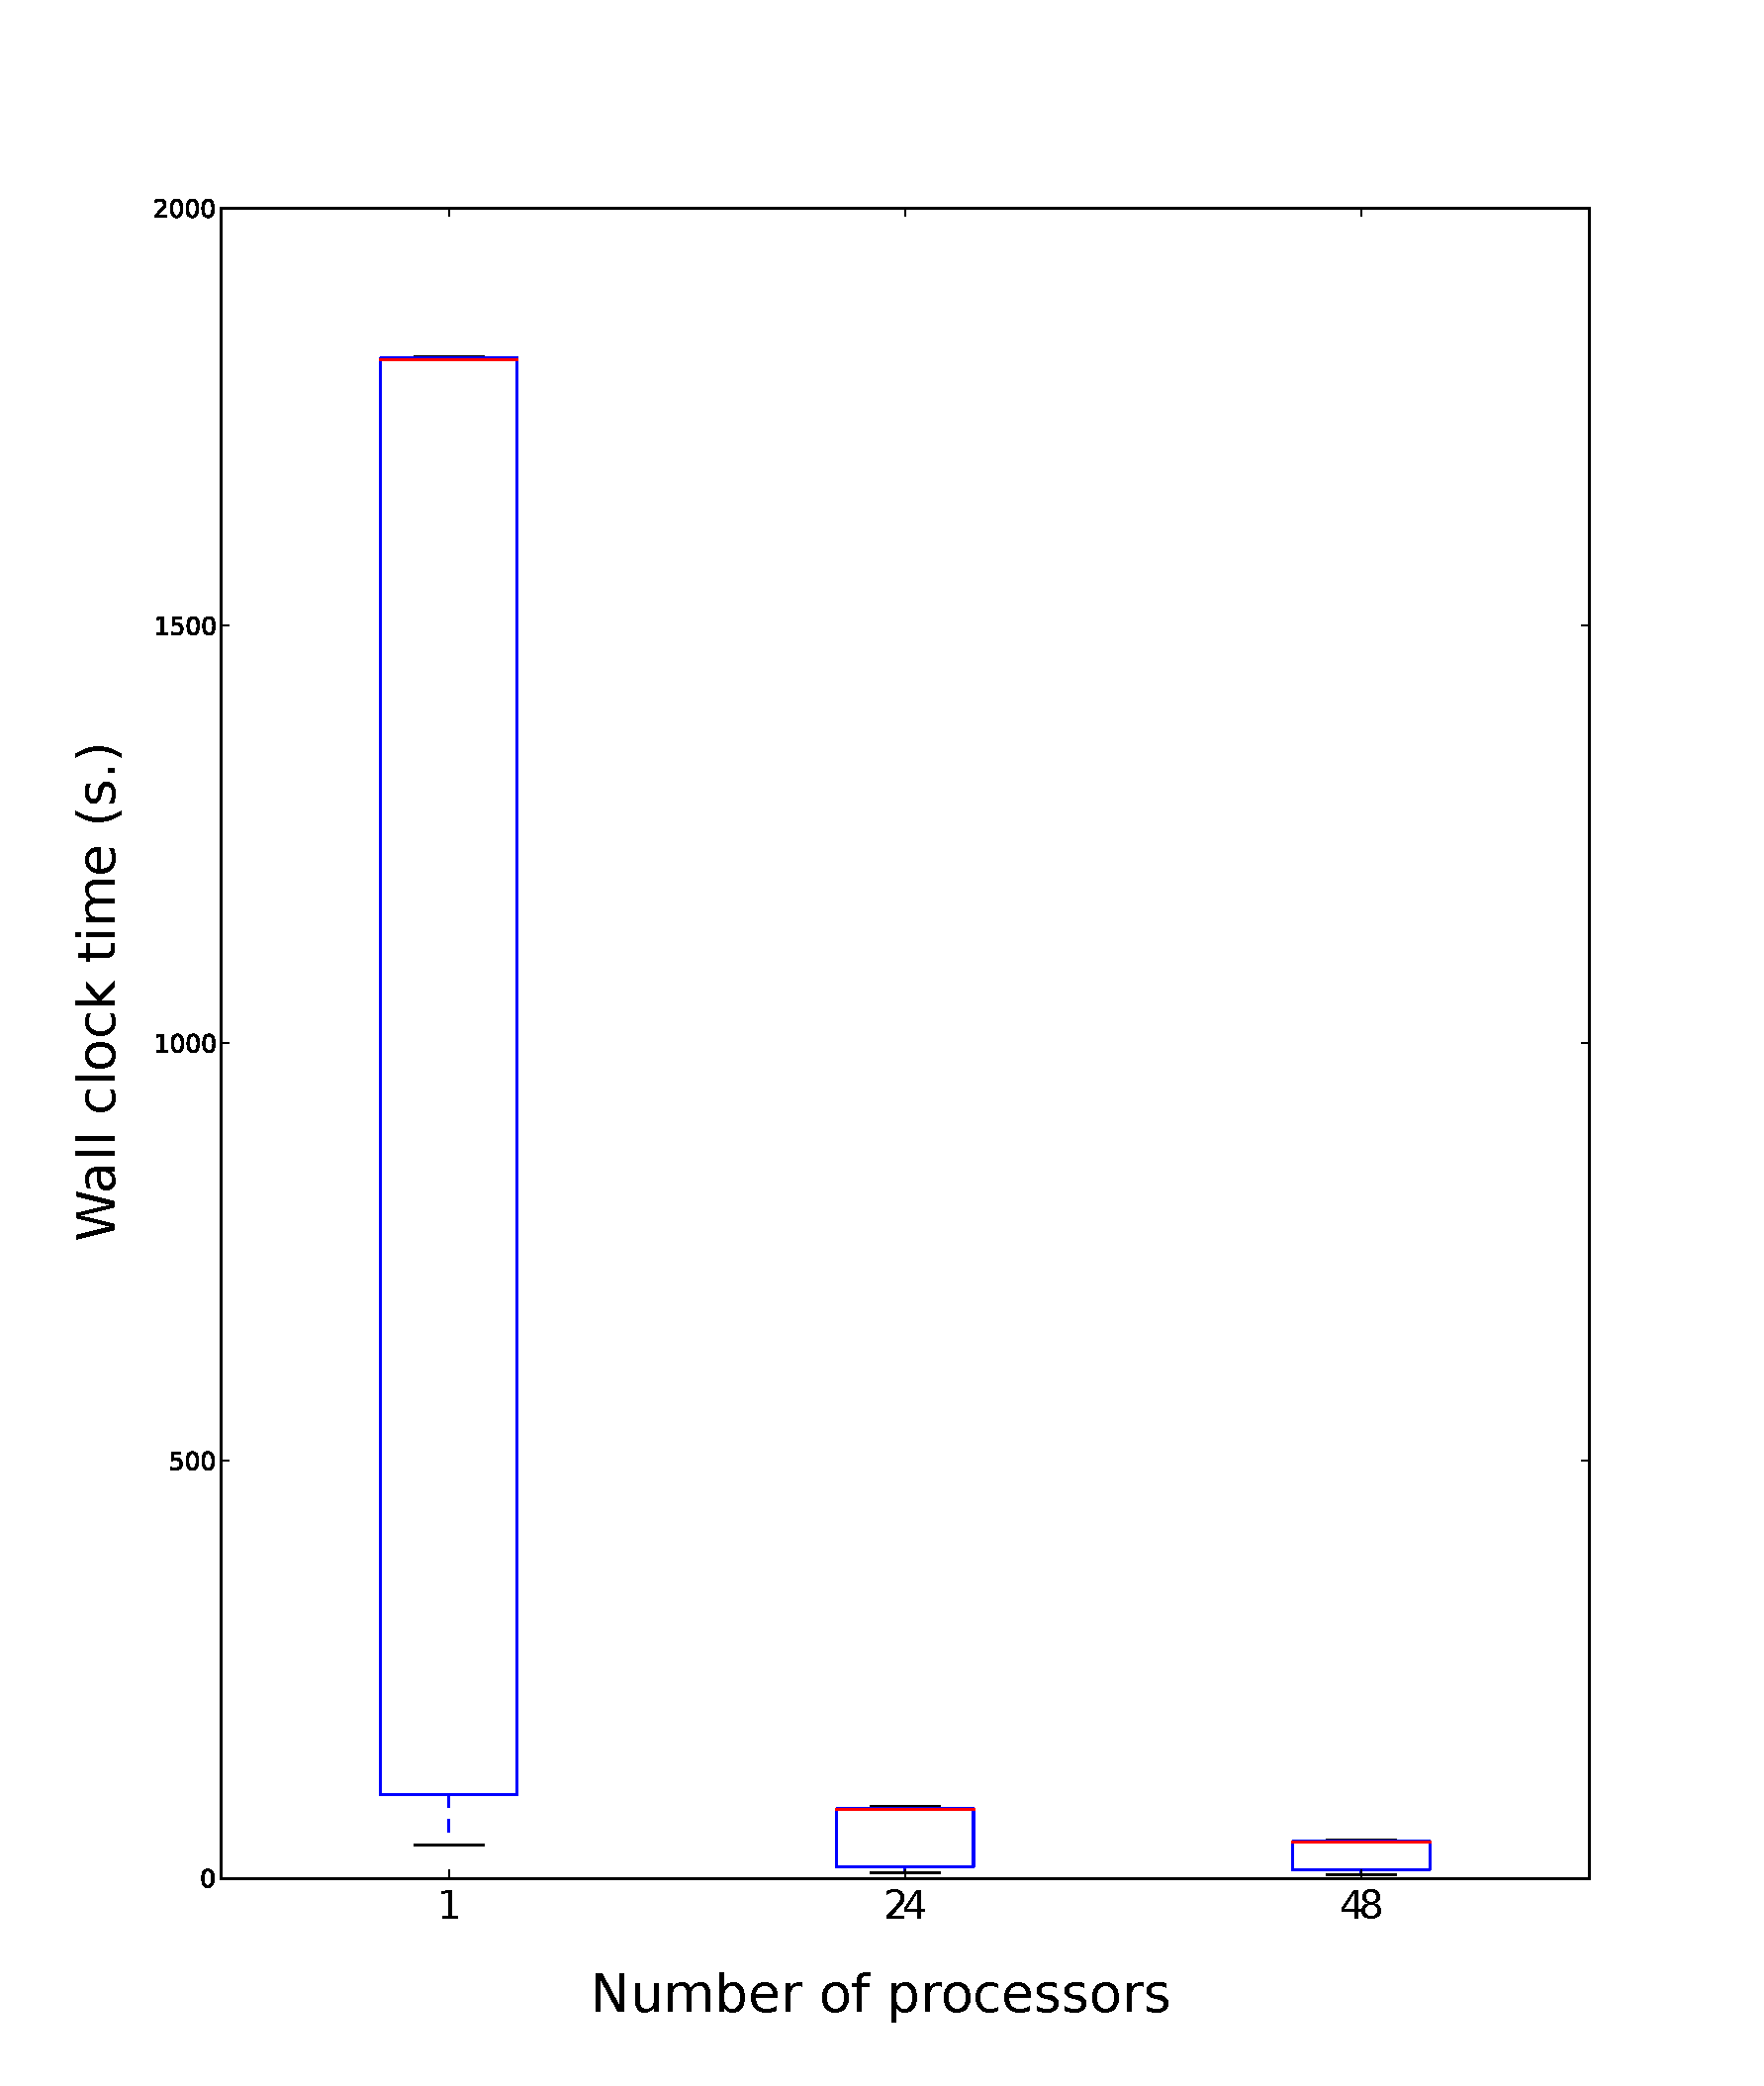
\includegraphics[width=0.23\textwidth]{images/elevators_proc_time.pdf}}
 \hfill
 \subfigure[\OPENSTACKS-17]{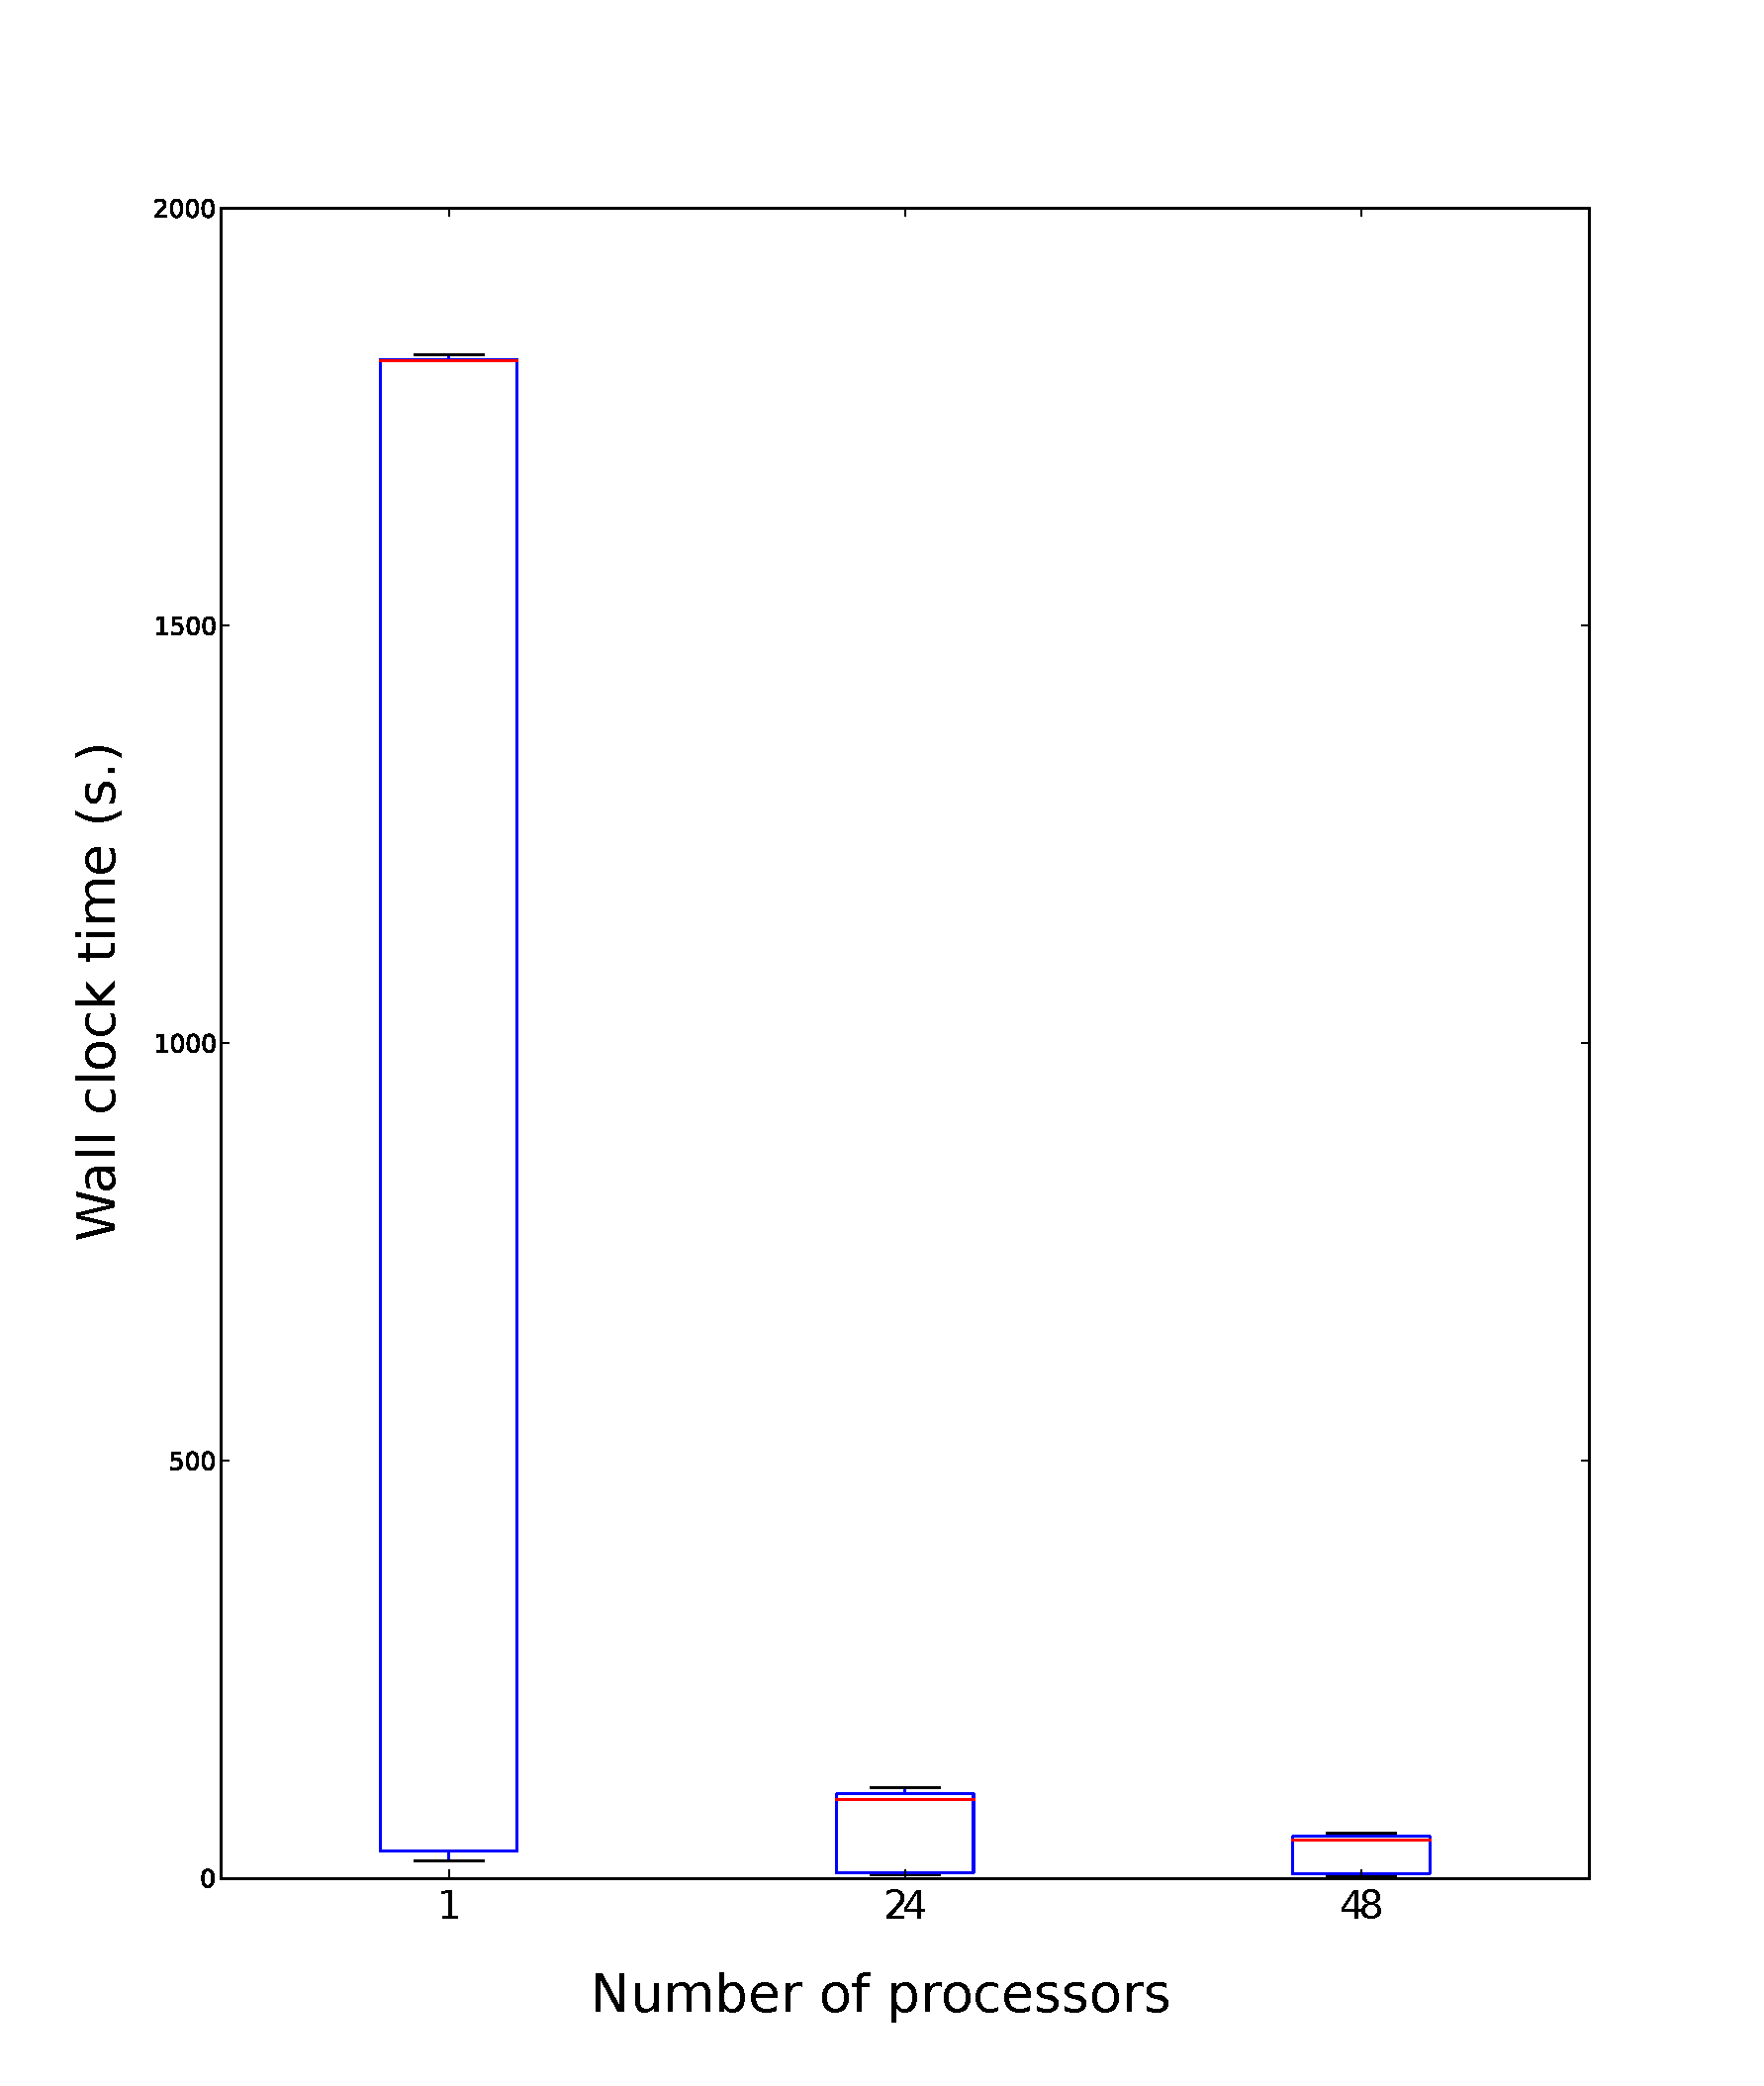
\includegraphics[width=0.23\textwidth]{images/openstacks_proc_time_dynamic.pdf}}
 \end{center}
 \caption{Wallclock time distributions of 11 runs of \DAEYAHSP\ relative to the number of processors used.}
 \label{fig:proc_elevators_vs_openstacks}
\end{figure}

Figure \ref{fig:proc_elevators_vs_openstacks} shows that on both problems, the
computation time decreases with the number of processors used. Comparing to the
sequential version (running on a single processor), the parallel one permit a
decrease that is similar on both problems. The dispersions of the distribution
is due to the steady-state stopping criterion that may be reached after different
times.

\paragraph{Comparison of Static and Dynamic Scheduling}
\OPENMP\ lets the choice between static and dynamic task scheduling. The default one is the static scheduling.
In the static scheduling, a loop iterating through a set of tasks will be
divided in several tasks relative to the number of available processors.
Regarding dynamic scheduling, during the runtime if one thread has finished
these tasks it gets the next available one, in a queue.

% some hypotheses

% on a pas teste tout �a en pratique
%Two hypotheses have driven us to test the dynamic scheduling. The first one consists to say that as long as we are using a problem solved in a variable time, the dynamic scheduling should be faster than the static scheduling does. The second one assumes that we use a population size higher than the number of cores available, the dynamic mode should bring a better efficiency.

% To determine the quality of the dynamicity in front of statical schedule, we
% are using the following formula:
% $$D_p = \frac{S^s_p}{S^d_p}$$
% $S^s_p$ is the speedup for the static scheduling.\\
% $S^d_p$ is the speedup for the dynamic one.\\

\begin{figure}[htpb]
 \begin{center}
 \subfigure[static]{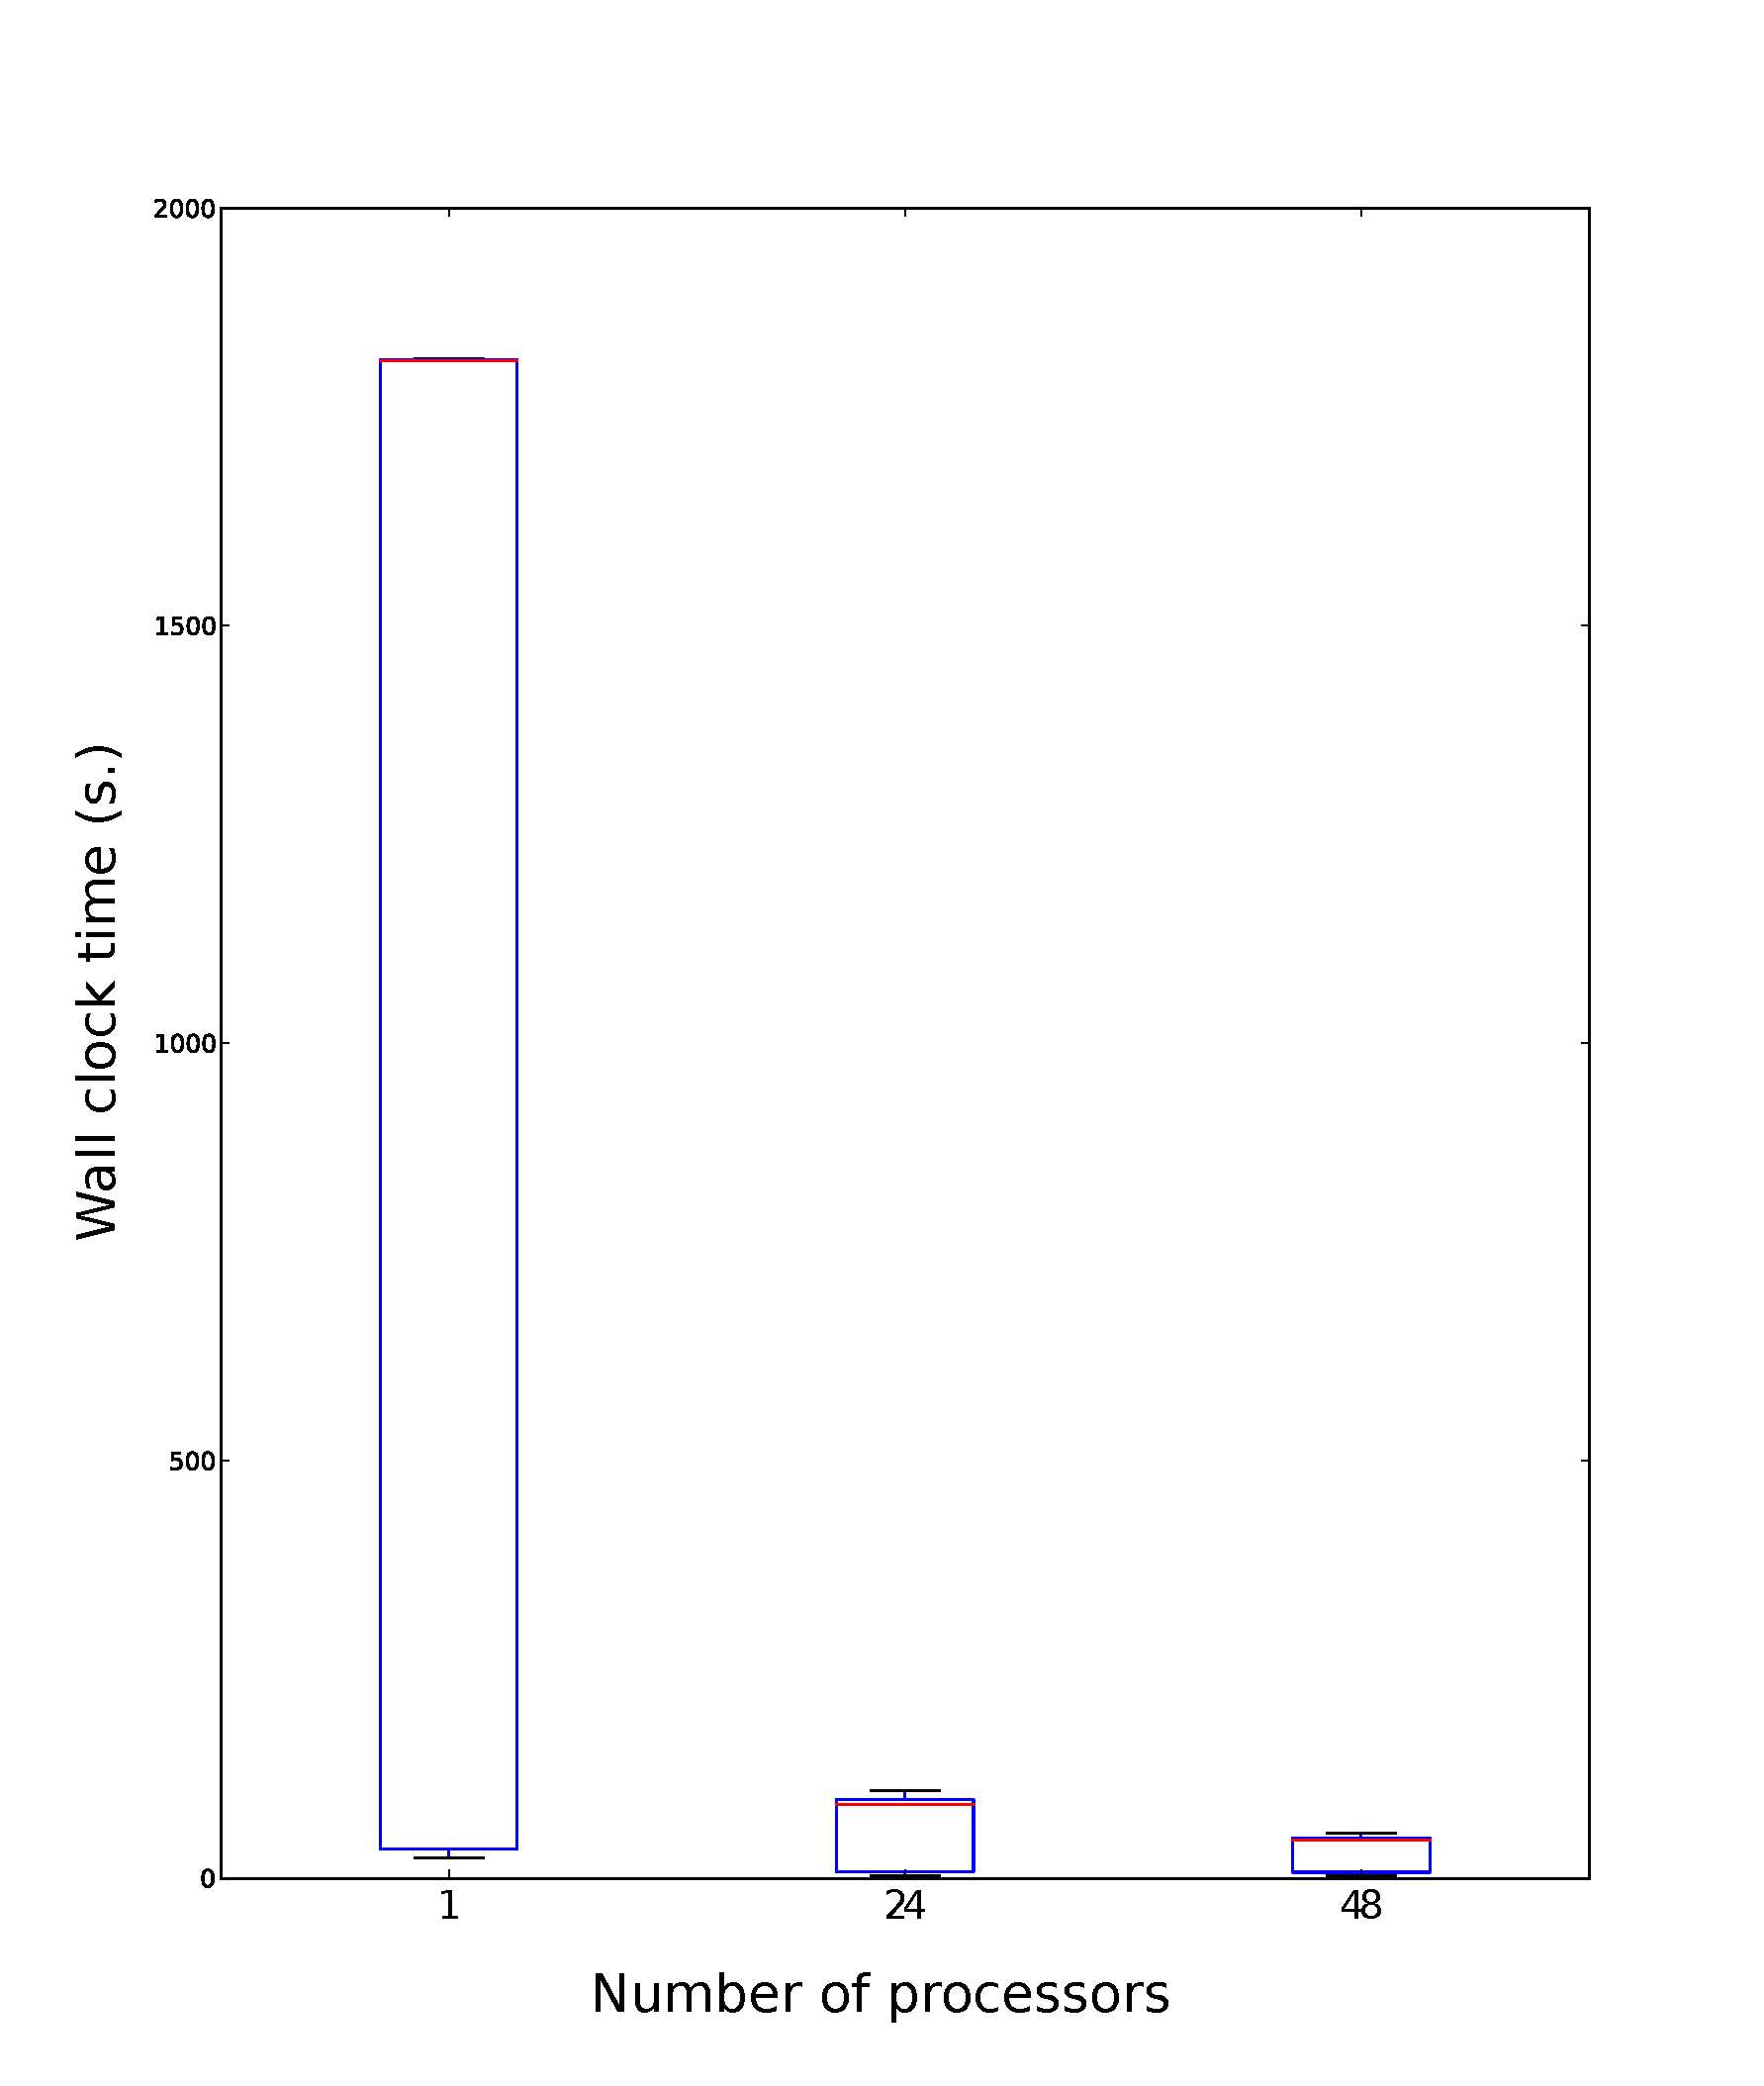
\includegraphics[width=0.23\textwidth]{images/openstacks_proc_time_static.pdf}}
 \hfill
 \subfigure[dynamic]{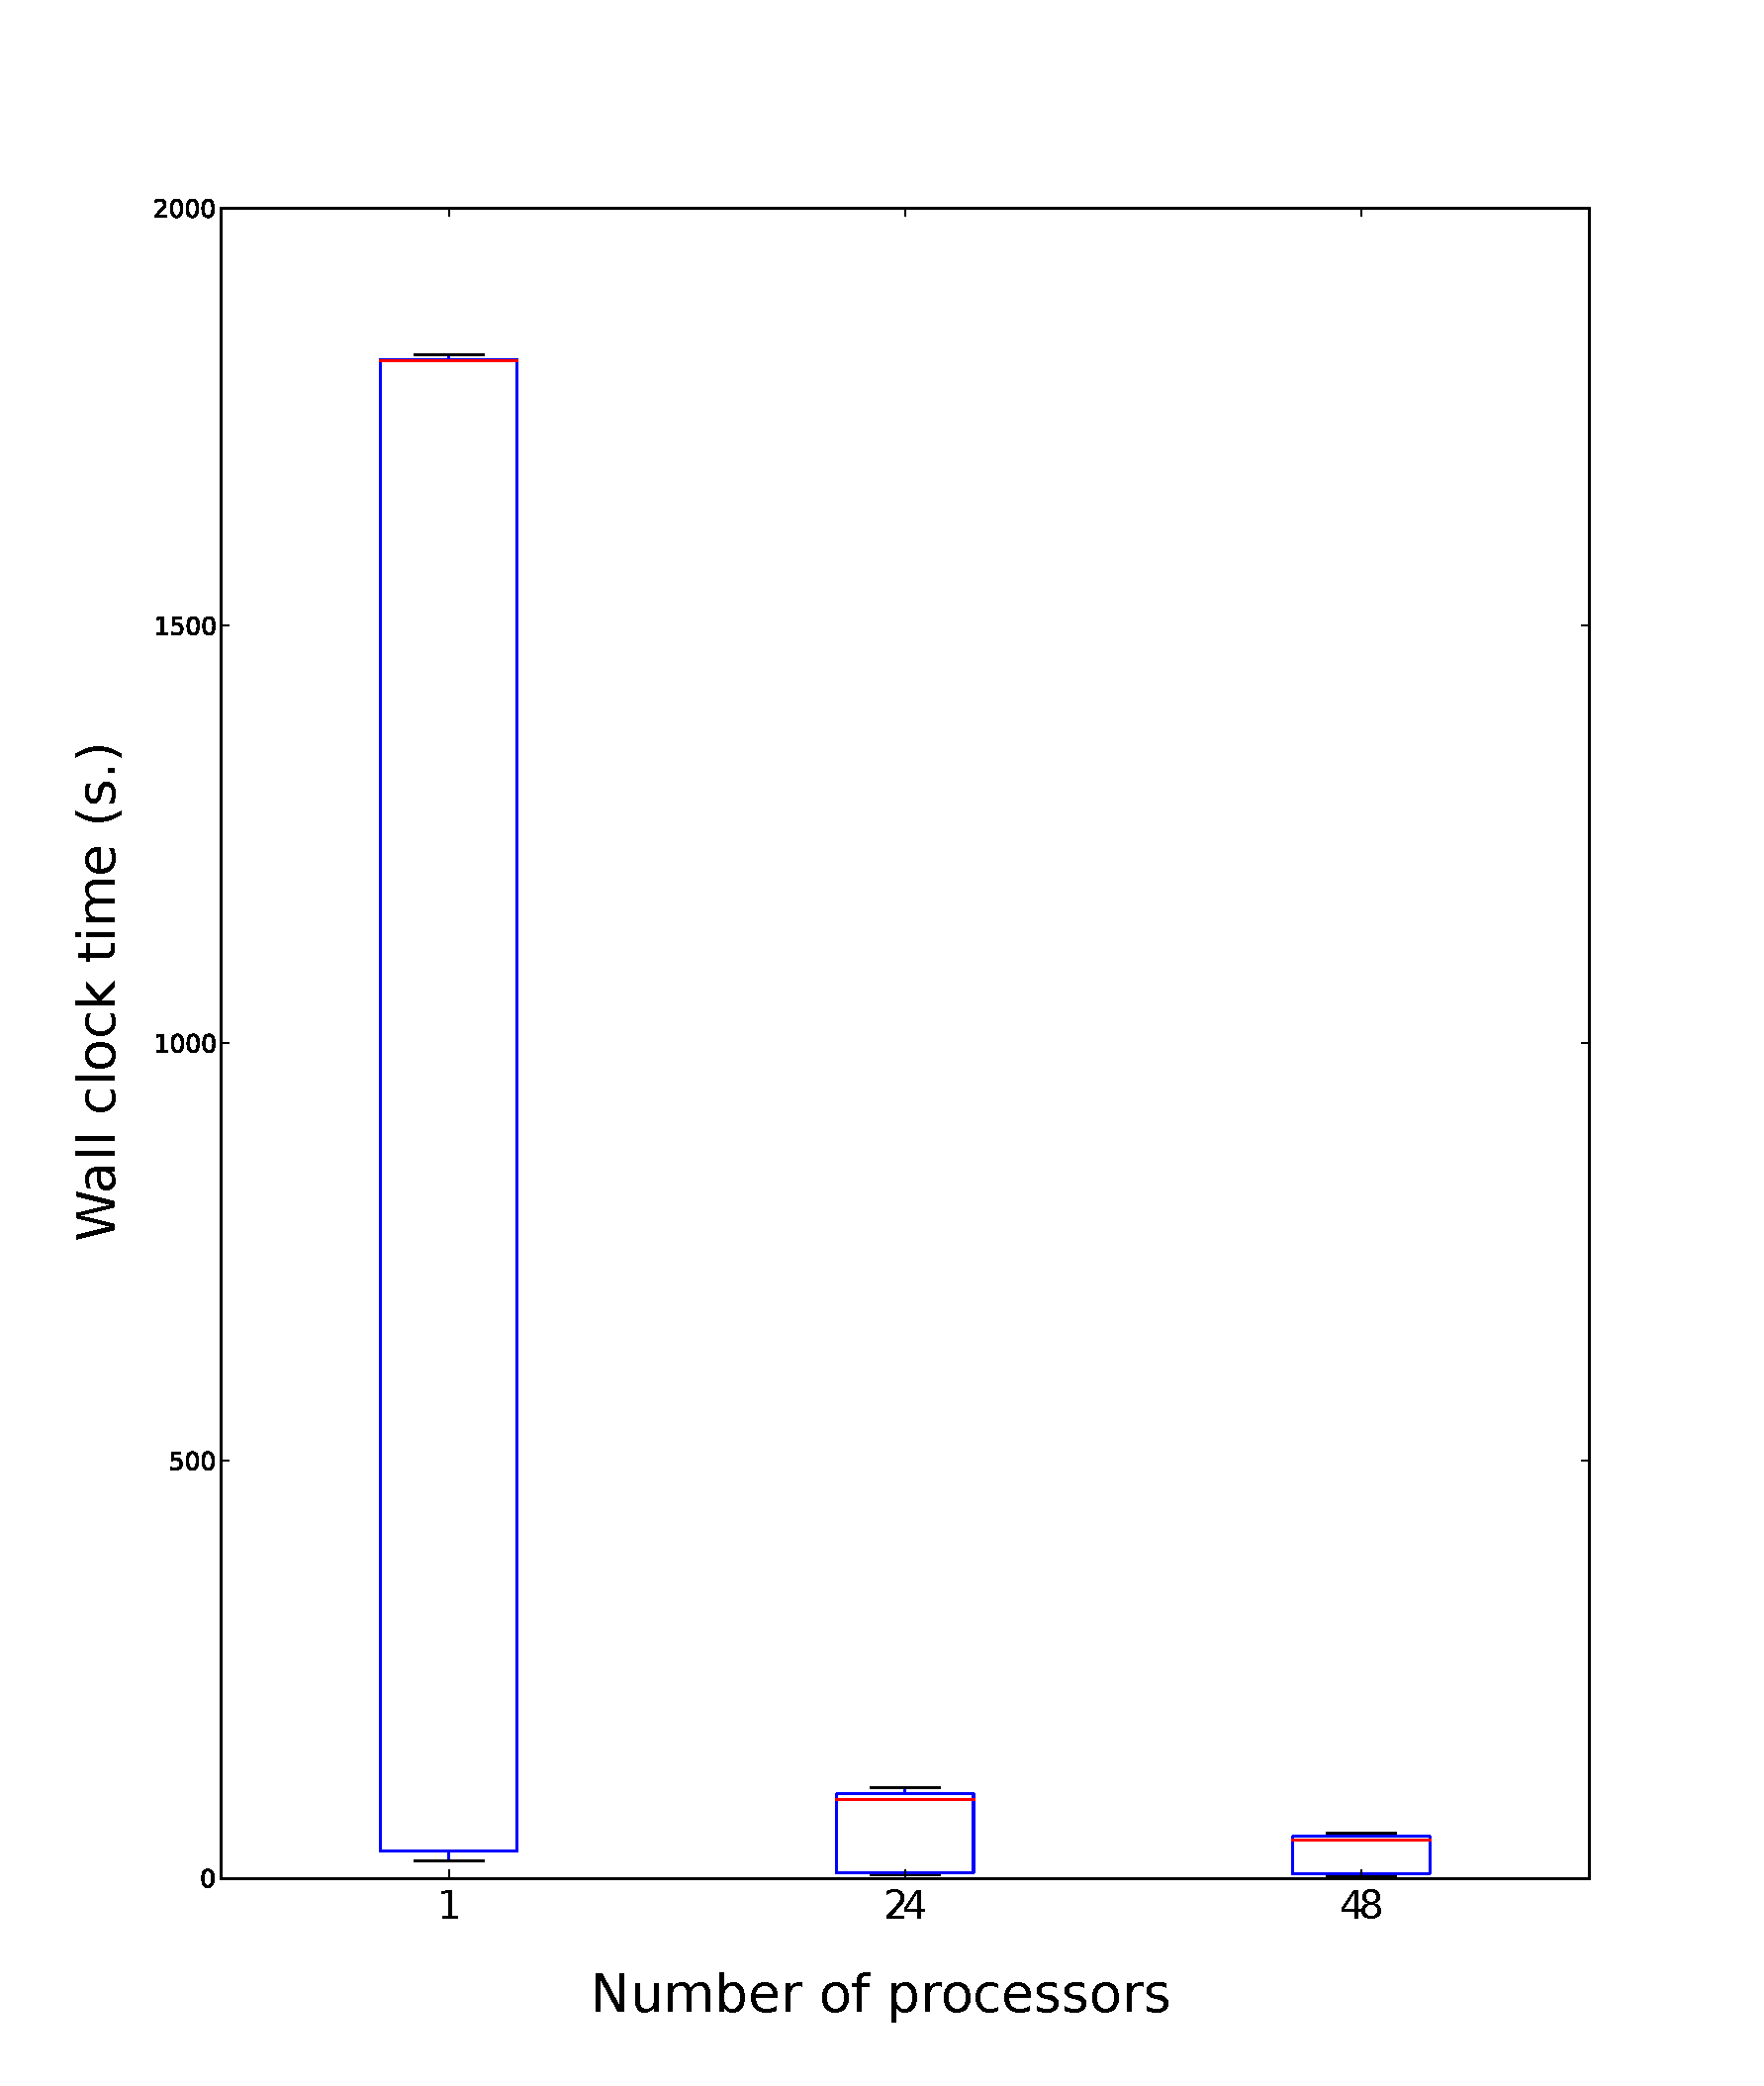
\includegraphics[width=0.23\textwidth]{images/openstacks_proc_time_dynamic.pdf}}
 \end{center}
 \caption{Wallclock time distributions of 11 runs of \DAEYAHSP\ relative to the number of processors, on the temporal \OPENSTACKS-17 problem.}
 \label{fig:proc_static_vs_dynamic}
\end{figure}

Figure \ref{fig:proc_static_vs_dynamic} shows that the dynamic parallelization
scheme does not permit a significant speed-up comparing to the static one. The
Wilcoxon signed-rank test cannot reject the null hypothesis that the samples come
from the same distribution ($p=0.03$).

\paragraph{Speed-up against the Population Size} % (CC, JD)

\begin{figure}[htpb]
 \begin{center}
 \subfigure[full scale]{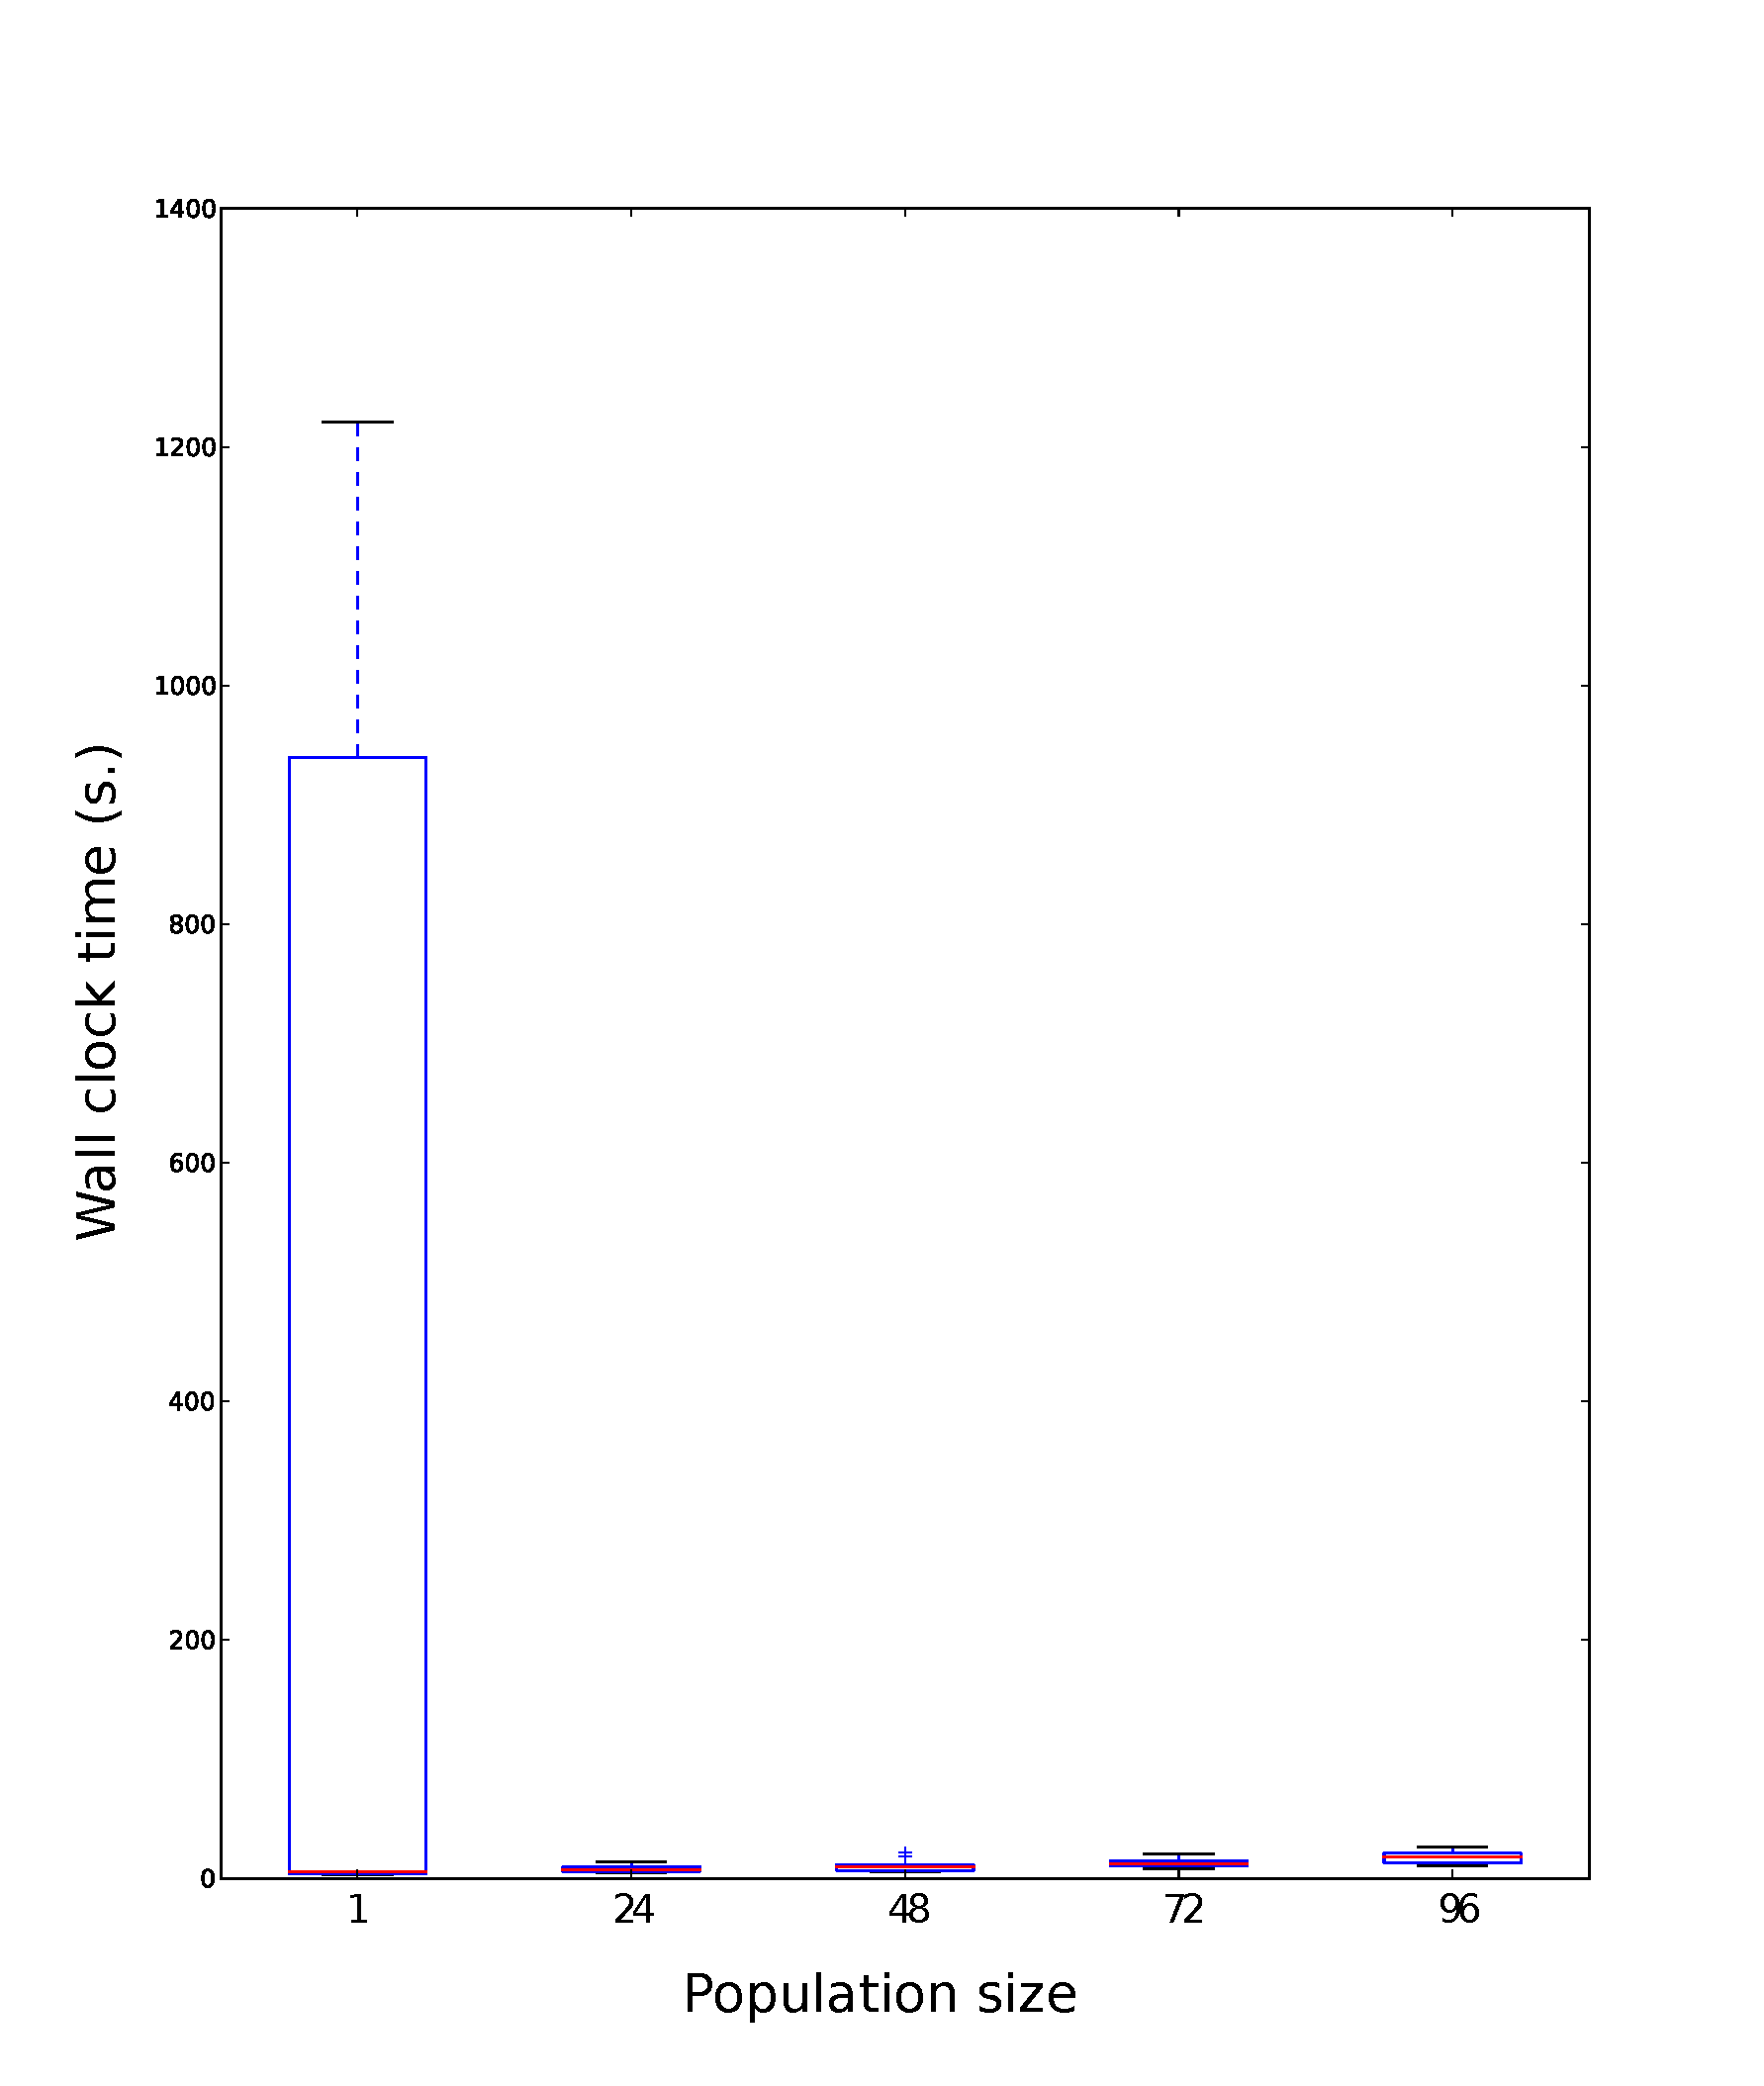
\includegraphics[width=0.23\textwidth]{images/elevators_pop_time.pdf}}
 \hfill
 \subfigure[rescaled]{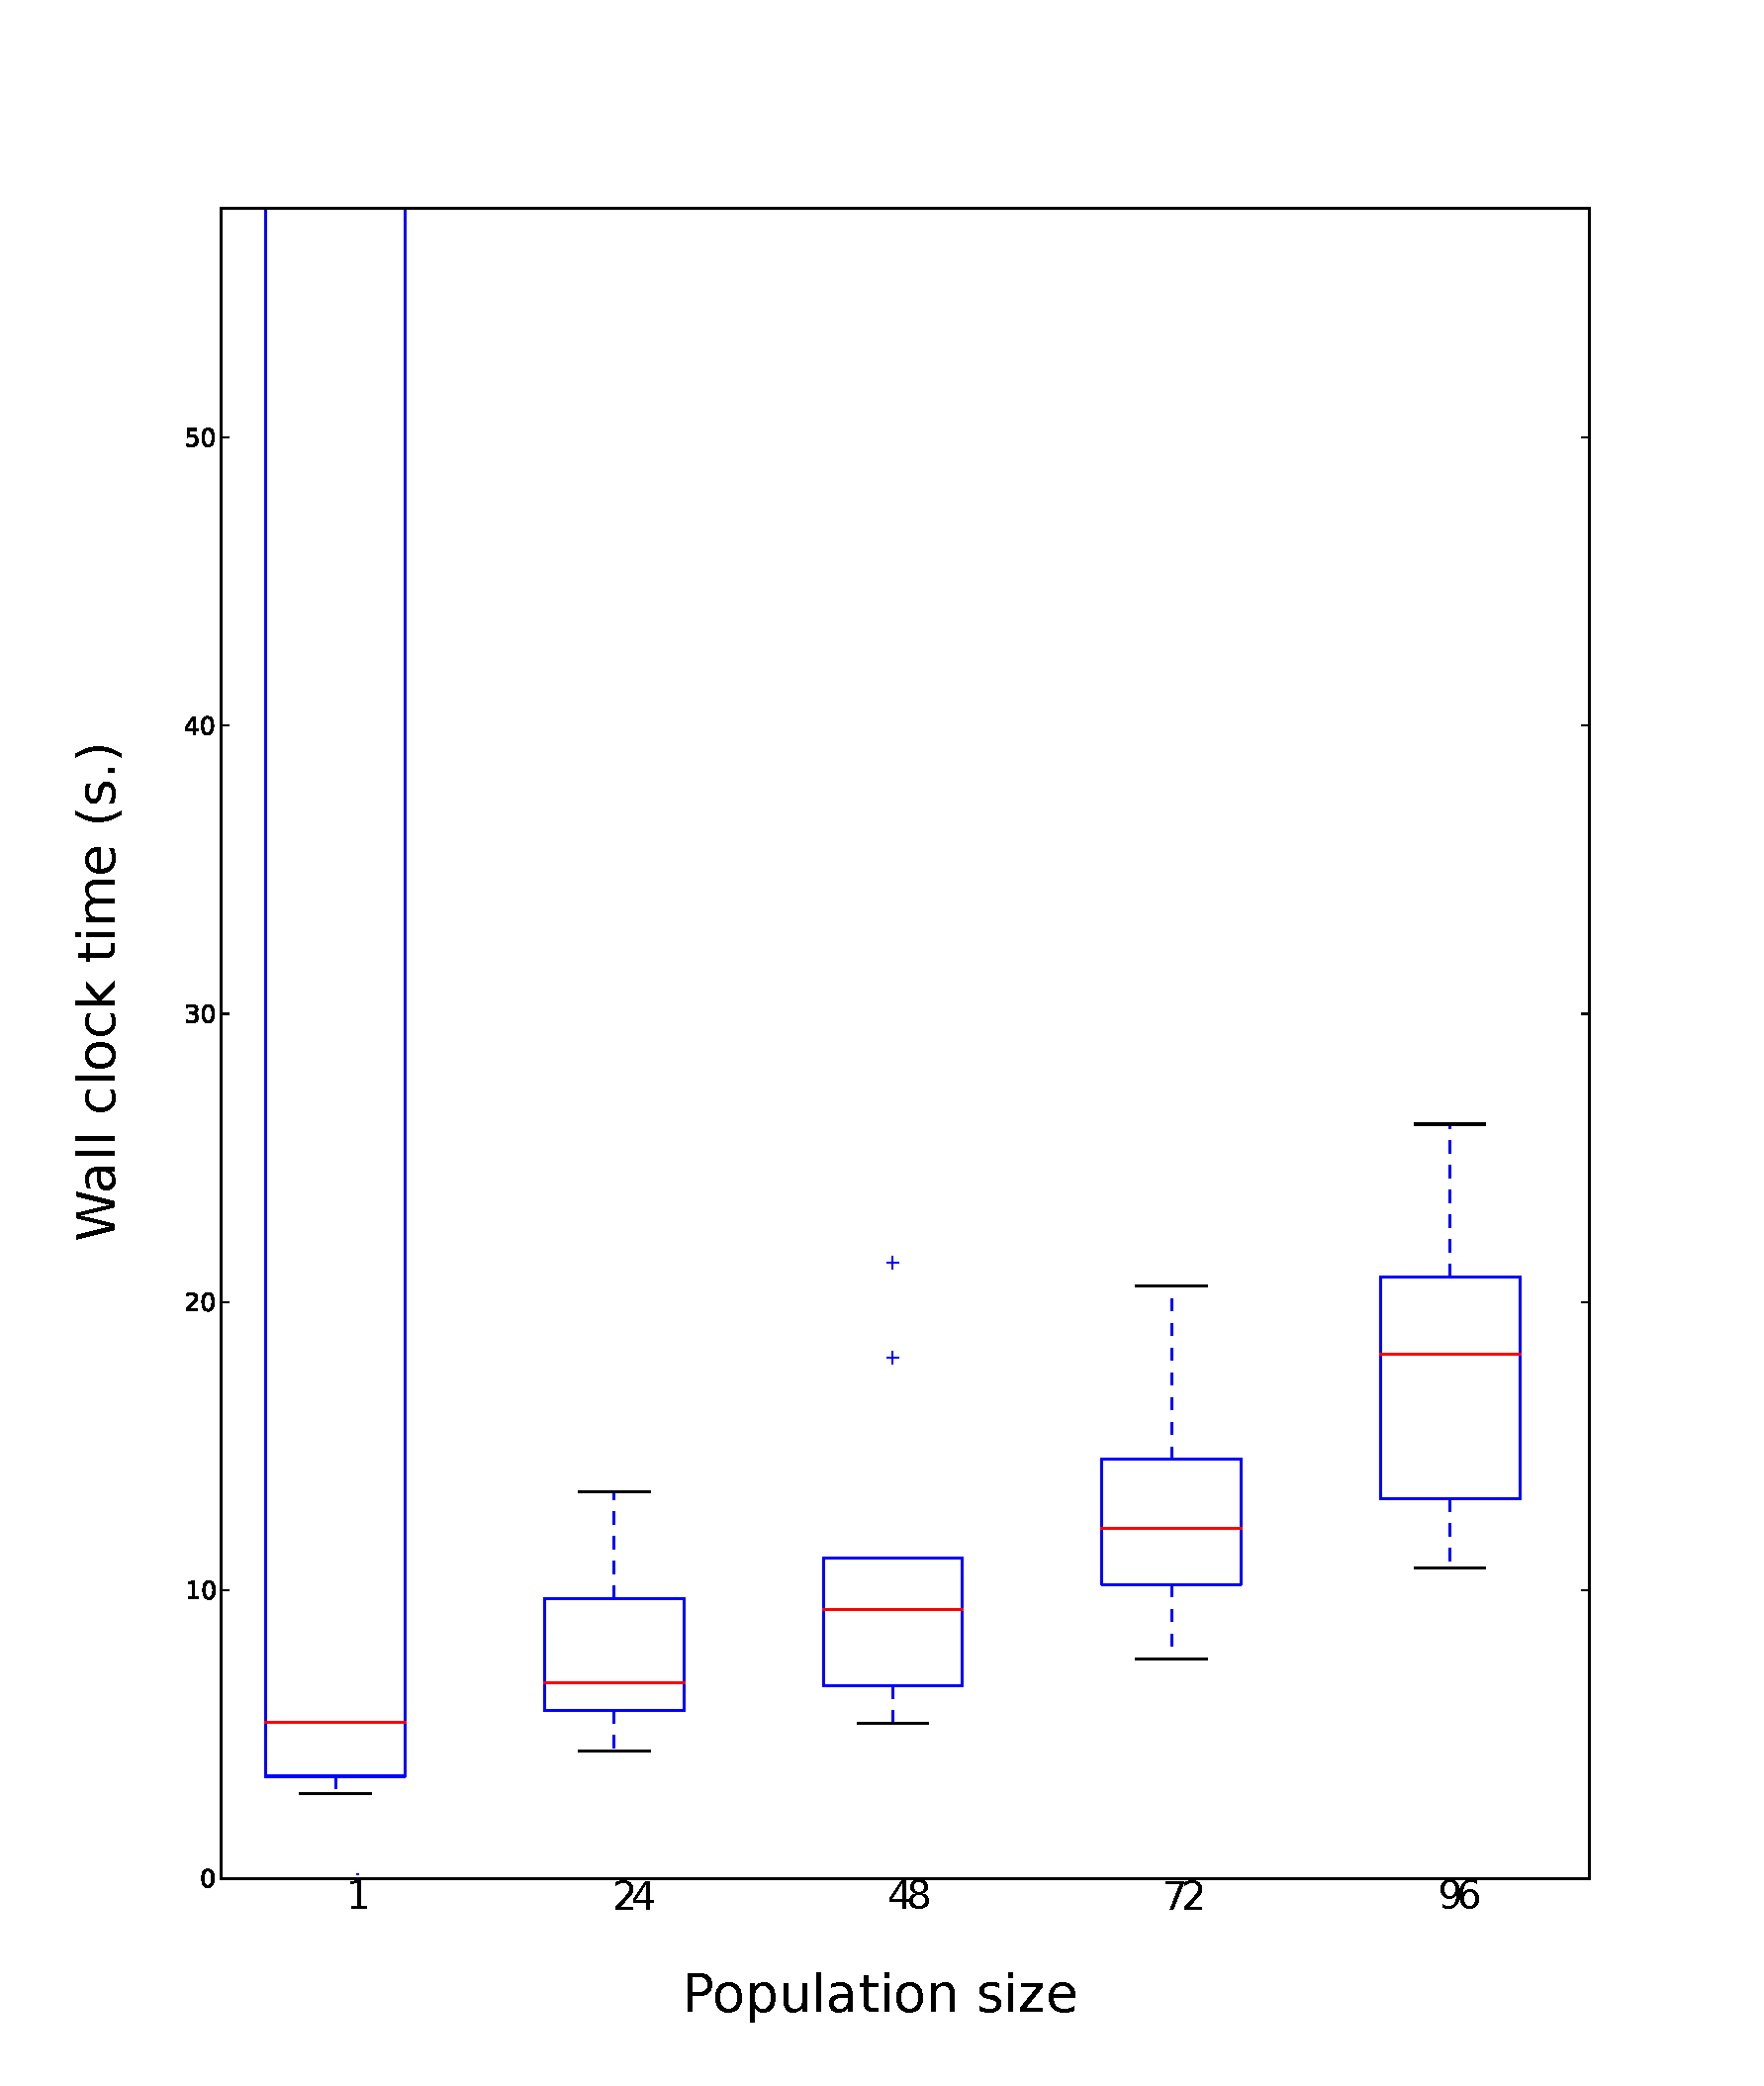
\includegraphics[width=0.23\textwidth]{images/elevators_pop_time_zoom.pdf}}
 \end{center}
 \caption{Wallclock time distributions of 11 runs of \DAEYAHSP\ relative to the population size, on the sequential \ELEVATORS-12 problem, using 48 processors.}
 \label{fig:elevators_pop}
\end{figure}

Figure \ref{fig:elevators_pop} shows that the median computation time on a multicore machine increases linearly with the size of the population. 
The dispersion of the distribution is due to the steady-state stopping criterion that may be reached after different times, with a higher probability when the
population size is small.

\begin{figure}[htpb]
 \begin{center}
 \subfigure[\ELEVATORS-12]{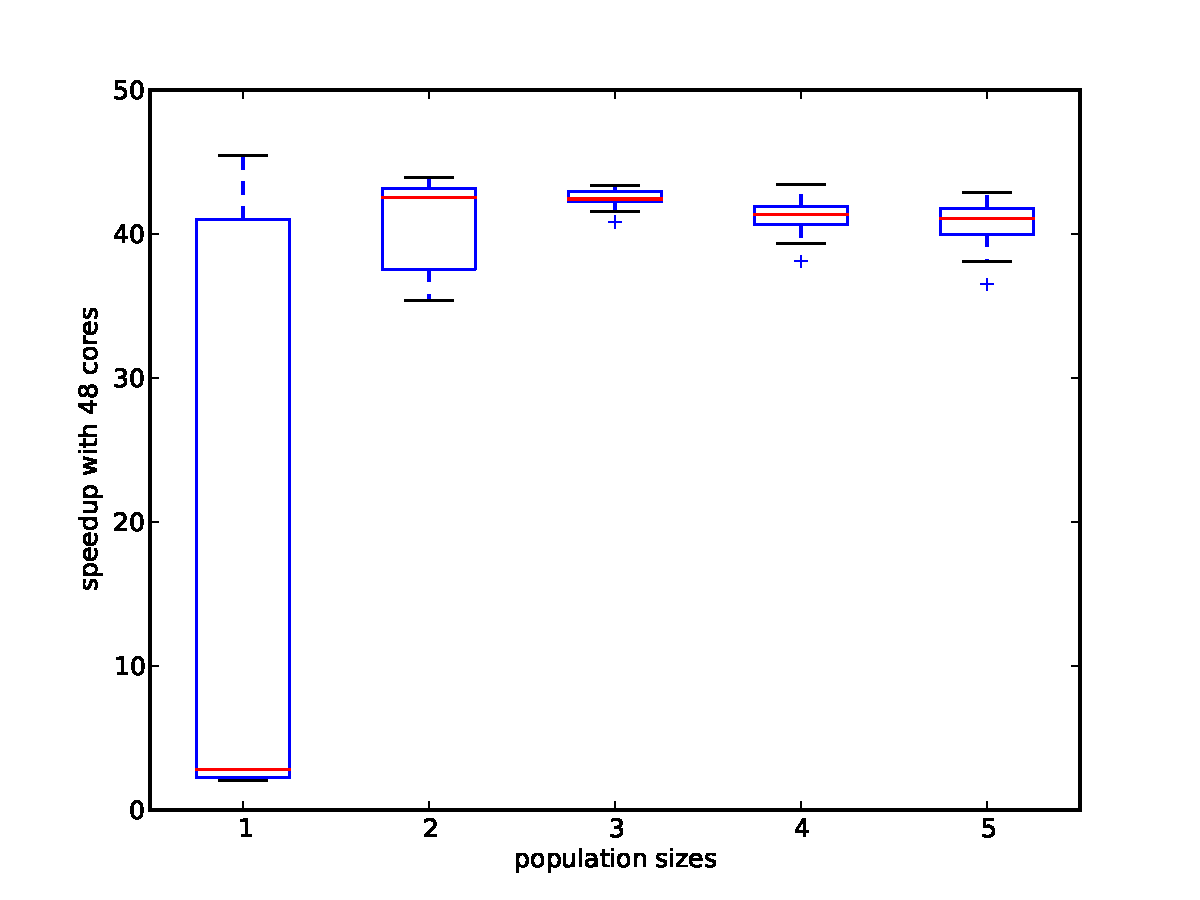
\includegraphics[width=0.23\textwidth]{images/elevators_pop_time_speedup.pdf}}
 \hfill
 \subfigure[\OPENSTACKS-17]{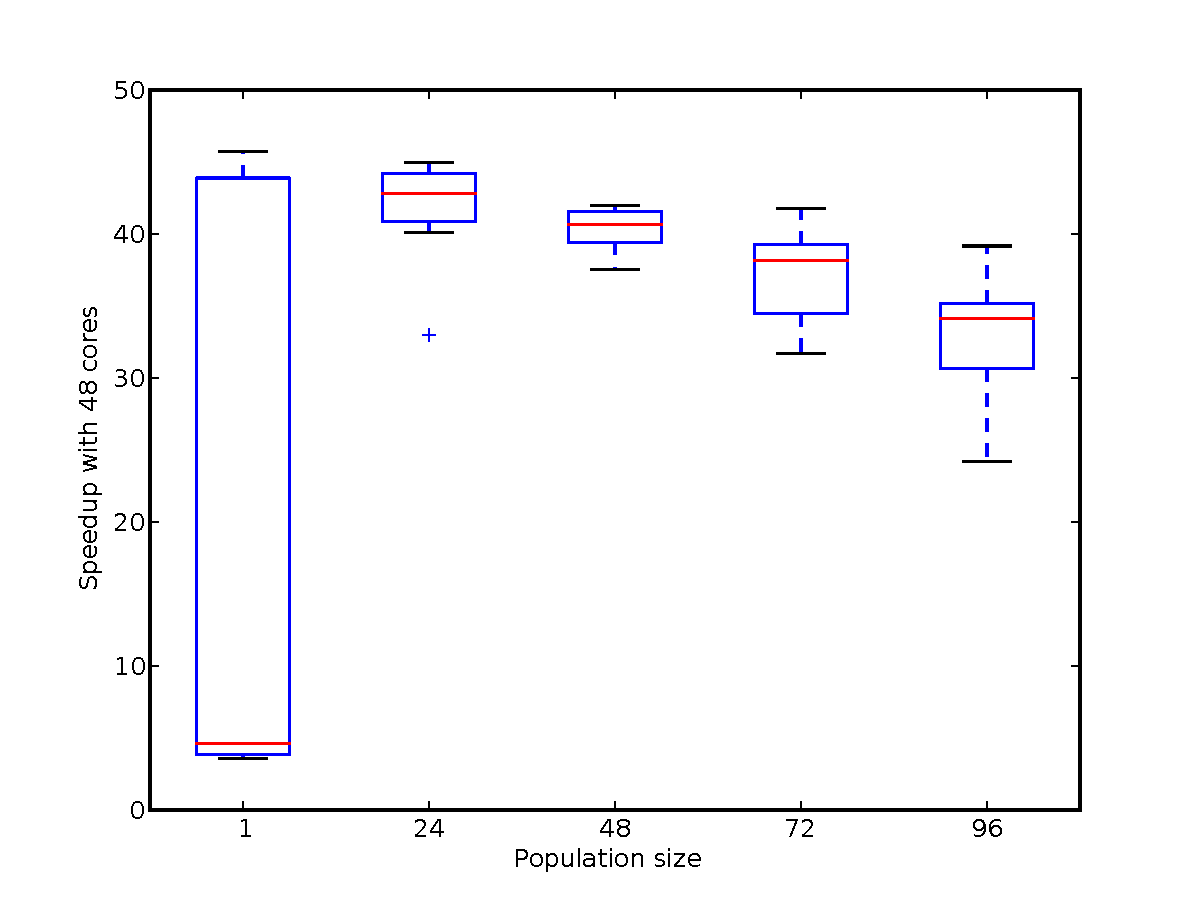
\includegraphics[width=0.23\textwidth]{images/openstacks_pop_time_speedup.pdf}}
 \end{center}
 \caption{Speedup distributions of 11 runs of \DAEYAHSP\ relative to the population size, on the both sequential \ELEVATORS-12 and temporal \OPENSTACKS-17 problems, using 48 processors.}
 \label{fig:speedup_pop}
\end{figure}

Figure \ref{fig:speedup_pop} shows that the expected speed-up of $40$ is met, and that it decrease with the population size. The measures were done according
to the speedup equation.

$$S_p = \frac{T^*_1}{T_p}$$

The parameters $T^*_1$ and $T_p$ are respectively the time used for a sequential and a parallel execution.

%%$$Speedup\ measure = r \sum^{P}_{k=0} \frac{T^*_{1_k}}{T_{p_k}}$$

\section{Discussion and Conclusion}
%In order to scale up the capabilities of \DAEYAHSP, this paper investigated the
%parallelization of the individual evaluation.

We made a proof-of-concept of a shared-memory parallelization of the evaluation
step of the \DAEX algorithm, based on the \OPENMP\ directive-based API on a common
48-core machine. Thanks to the abstraction level provided by the EO framework,
this scheme is immediately available for any evolutionary algorithm as far as
the context of the evaluation functor is thread-local and reentrant.

As expected, on our 48-core Dell Machine a roughly $\times40$ speed-up was obtained on
the tested benchmark, this speed-up being the same for all instances.

The dispersion of the measured times is mainly due to the
combination of the steady-state stopping criterion with the stochastic nature
of the search, which may or may not reach a fitness plateau early. The
relationship between this dispersion and the hardness of the problem solved
remains to be explored.

Our results show that the stopping criterion should be chosen carefully, along
with the population size, as it has an impact on the dispersion of the
distribution of computation times.

The dynamic queue mapping management of threads onto cores did not provide a significant
improvement. Our hypothesis was that the goal sequences shows a diversity in
length and thus should have shown very diverse times of evaluation computations.
But we observed that the algorithm converges rapidly to a same length for all
individuals.

The implementation scheme presented here is very simple, but works extremely
well. A further development will consist in parallelizing other steps of the
evolutionary loop in particular the offspring generation which is also
intrinsically parallel, as it use independent variation operators.

% FIX ME Further research: adapting the YAHSP memoing feature to the
% parallelization scheme : 2 modes global vs local memoing

% Impact on the EA design
% Do you agree below?
A further research axis deals with the impact on solution quality and in
particular how to take advantage of the parallelization scheme to escape from
premature convergence.

\section{Acknowledgments}
This work is being partially funded by the French National Research Agency through the COSINUS programme, under the research contract DESCARWIN (ANR-09-COSI-002).


%
% The following two commands are all you need in the
% initial runs of your .tex file to
% produce the bibliography for the citations in your paper.
\bibliographystyle{abbrv}
\bibliography{dae_mt} % sigproc.bib is the name of the Bibliography in this case
% You must have a proper ".bib" file
% and remember to run:
% latex bibtex latex latex
% to resolve all references
%
% ACM needs 'a single self-contained file'!
%
%Generated by bibtex from your ~.bib file. Run latex,
%then bibtex, then latex twice (to resolve references)
%to create the ~.bbl file. Insert that ~.bbl file into
%the .tex source file and comment out
%the command \texttt{{\char'134}thebibliography}.
\end{document}
%
%\DAE\ has been implemented within the Evolving Objects framework (\url{http://eodev.sourceforge.net/}), an Open Source, STL-based, C++ Evolutionary Computation library.
%The fixed {\em evolution engine} is a (100+700)-ES: 100 individuals generate 700 offsprings without selection. The survival selection is performed among those 800 individuals using a {\em deterministic tournament} of size 5. For all runs, the {\bf stopping criterion} is the following: After at least 10 generations, evolution is stopped if no improvement of the best fitness in the population is made during 50 generations, with a maximum of 1000 generations. Furthermore, all runs were allowed a maximum CPU time of 30mn (running on 3.4 GHz cores).
%
%
%Multicore machines are becoming a standard way to speep up the system performance.
%
%This paper describes a multi-threaded release of \DAEYAHSP.
%
%This paper describes a parallel shared-memory release of the \DAEYAHSP\ planning system.
%using the \OPENMP\ directive-based API.
%
%to obtain high levels of performance special care has been given to get reentrant procedures.
%isolate context variables
%
% concurrent programming
%
%\OPENMP\ primarily consists of a set of compiler directives (pragmas) that are inserted into a Fortran, C or C++ program to convey information to an \OPENMP\ compiler.

%
%In order to scale up the capabilities of \DAEYAHSP, this paper investigated the parallelization of the individual evaluation.
